%%%%%%%%%%%%%%%%%%%%%%%% file template.tex %%%%%%%%%%%%%%%%%%%%%%%%%
%%
%% This is a general template file for the LaTeX package SVJour3
%% for Springer journals.          Springer Heidelberg 2010/09/16
%%
%% Copy it to a new file with a new name and use it as the basis
%% for your article. Delete % signs as needed.
%%
%% This template includes a few options for different layouts and
%% content for various journals. Please consult a previous issue of
%% your journal as needed.
%%
%%%%%%%%%%%%%%%%%%%%%%%%%%%%%%%%%%%%%%%%%%%%%%%%%%%%%%%%%%%%%%%%%%%%
%%
%% First comes an example EPS file -- just ignore it and
%% proceed on the \documentclass line
%% your LaTeX will extract the file if required
%\begin{filecontents*}{example.eps}
%%!PS-Adobe-3.0 EPSF-3.0
%%%BoundingBox: 19 19 221 221
%%%CreationDate: Mon Sep 29 1997
%%%Creator: programmed by hand (JK)
%%%EndComments
%gsave
%newpath
%  20 20 moveto
%  20 220 lineto
%  220 220 lineto
%  220 20 lineto
%closepath
%2 setlinewidth
%gsave
%  .4 setgray fill
%grestore
%stroke
%grestore
%\end{filecontents*}
%%
%\RequirePackage{fix-cm}
%%
%%\documentclass{svjour3}                     % onecolumn (standard format)
%%\documentclass[smallcondensed]{svjour3}     % onecolumn (ditto)
%%\documentclass[smallextended]{svjour3}       % onecolumn (second format)


\documentclass[twocolumn]{svjour3}          % twocolumn
%
\smartqed  % flush right qed marks, e.g. at end of proof
%
\usepackage{amssymb}
\usepackage{caption}
\usepackage{slashbox}
\usepackage{graphics} % for pdf, bitmapped graphics files
\usepackage{epsfig} % for postscript graphics files
\usepackage{epstopdf}
\usepackage{subfig}
\usepackage{mathptmx} % assumes new font selection scheme installed
\usepackage{amsmath} % assumes amsmath package installed
\usepackage{amsmath}
\usepackage{array}
\usepackage{bm}
\usepackage{multirow}
\usepackage[usenames,dvipsnames,svgnames,table]{xcolor}
\usepackage{pbox}
\usepackage{hyperref}
\usepackage{algorithm}
\usepackage{algpseudocode}
\usepackage{natbib}

\definecolor{light-gray}{gray}{0.8}

\begin{document}\sloppy

\title{A Modular Approach to Learning Manipulation Strategies from
  Human Demonstration}\thanks{Aude, do we need to acknowledge a funder?}
%}

%\subtitle{Do you have a subtitle?\\ If so, write it here}
%\titlerunning{Short form of title}        % if too long for running head
\author{Authors        \and
        Authors %etc.
}
%\authorrunning{Short form of author list} % if too long for running head
%\institute{F. Author \at
%              first address \\
%              Tel.: +123-45-678910\\
%              Fax: +123-45-678910\\
%              \email{fauthor@example.com}           %  \\
%%             \emph{Present address:} of F. Author  %  if needed
%           \and
%           S. Author \at
%              second address
%}

%\date{Received: date / Accepted: date}
% The correct dates will be entered by the editor


\maketitle

\begin{abstract}
  Object manipulation is a challenging task for robotics as the
  physics involved in object interaction is complex and hard to
  express analytically. Here we introduce a modular approach for
  learning a manipulation strategy from human demonstration. After
  recording a human demonstrating the task in different contexts, we
  perform modular decomposition of the control strategy, using phases
  of the recorded actions to guide segmentation. Each module
  represents a part of the strategy, encoded as a pair of forward and
  inverse models. All modules contribute to the final control policy;
  their recommendations are integrated via a system of weighting based
  on their own estimated error in the current task context. We
  validate our approach by demonstrating it on a robot platform.  The
  task is opening a bottle cap. We show that our approach can
  modularize an adaptive control strategy to generate appropriate
  motor commands for the robot to accomplish the complete task. 
%\keywords{First keyword \and Second keyword \and More}
% \PACS{PACS code1 \and PACS code2 \and more}
% \subclass{MSC code1 \and MSC code2 \and more}
\end{abstract}



%\section{Introduction}
%\label{intro}
%Your text comes here. Separate text sections with
%\section{Section title}
%\label{sec:1}
%Text with citations \cite{RefB} and \cite{RefJ}.
%\subsection{Subsection title}
%\label{sec:2}
%as required. Don't forget to give each section
%and subsection a unique label (see Sect.~\ref{sec:1}).
%\paragraph{Paragraph headings} Use paragraph headings as needed.
%\begin{equation}
%a^2+b^2=c^2
%\end{equation}
%
%% For one-column wide figures use
%\begin{figure}
%% Use the relevant command to insert your figure file.
%% For example, with the graphicx package use
%  \includegraphics{example.eps}
%% figure caption is below the figure
%\caption{Please write your figure caption here}
%\label{fig:1}       % Give a unique label
%\end{figure}
%%
%% For two-column wide figures use
%\begin{figure*}
%% Use the relevant command to insert your figure file.
%% For example, with the graphicx package use
%  \includegraphics[width=0.75\textwidth]{example.eps}
%% figure caption is below the figure
%\caption{Please write your figure caption here}
%\label{fig:2}       % Give a unique label
%\end{figure*}
%%
%% For tables use
%\begin{table}
%% table caption is above the table
%\caption{Please write your table caption here}
%\label{tab:1}       % Give a unique label
%% For LaTeX tables use
%\begin{tabular}{lll}
%\hline\noalign{\smallskip}
%first & second & third  \\
%\noalign{\smallskip}\hline\noalign{\smallskip}
%number & number & number \\
%number & number & number \\
%\noalign{\smallskip}\hline
%\end{tabular}
%\end{table}


%\begin{acknowledgements}
%If you'd like to thank anyone, place your comments here
%and remove the percent signs.
%\end{acknowledgements}

% BibTeX users please use one of
%\bibliographystyle{spbasic}      % basic style, author-year citations
%\bibliographystyle{spmpsci}      % mathematics and physical sciences
%\bibliographystyle{spphys}       % APS-like style for physics
%\bibliography{}   % name your BibTeX data base

\section{Introduction}
\label{intro}
%The ultimate goal of robotics is to enable robots to be a part of human life, to provide assistance in a wide range of tasks including surgery operation, house keeping, education and personal care. Most of these tasks require the ability to do complex object manipulation, which remains a open challenge in the robotics community. %It is impractical to pre-program all such object manipulation tasks manually. Therefore, we use a more practical alternative: teaching the robots by human demonstrations of the tasks.

With robots moving into human-centered environments such as households
and offices, human-like motor skills are becoming increasingly
desirable. In everyday life, object manipulation is one of the most
commonly used manual skills. Object manipulation includes a large
category of activities ranging from the simple pick-and-place task to
complicated dexterous manipulation.

Here we provide a framework for learning a human object-manipulation skill
and transferring it to a robot.
%Object manipulation is a large category of tasks in which the robots make physical contact with the environment. %Typical contact tasks include robot grasping and object manipulation.
%% The complicated physics in the interactions between objects makes manipulation tasks difficult. The multi-body interaction and the effect of friction can cause abrupt changes in the environment. To handle these situations, robots have to be equipped with a nonlinear and non-stationary control strategy, which is hard to design by analytical approaches.
%In manipulation tasks, the ability to predict and react to the uncertainty and unforeseen changes of the environment is vital.
Generally, manipulation tasks are very difficult, due to the
complicated contact situations between the manipulator and the object,
and the changing kinematic and dynamic contexts that result. Humans
can perform these skilled tasks and adapt to changes in context
without difficulty. At the heart of this skill is
prediction~\citep{flanagan2006control}. Studies from neuroscience
suggest that humans develop internal models for motor control, which
allow us to predict the future state of the environment. By comparing
the predictive state with the actual sensory state, the internal
models monitor the progression of  tasks, and launch any
corresponding motor correction and motor reaction required to
adapt to anything unexpected. %Building accurate analytical model for manipulation task is painstaking, small error in the model will cause fatal control problem. To solve this problem, we take the programming by human demonstration (PbD) approach.  %Modular approach has also been shown to be an effective way of building intelligent systems~\citep{bryson2004modular,BrysonMcG12}.

Inspired by this concept, we propose an approach to learn human
adaptive control strategy, \textcolor{red}{i.e. how to apply force or torque to accomplish a task according to the task context. By task context we mean  the dominant factors that will effect the performance of the task, e.g. frictions, object sizes and masses.} The adaptive control strategy is modeled by a modular approach. 
\textcolor{red}{The key concept of this modular approach is to decompose the adaptive control strategy into several modules and make them contribute accordingly to generate the final control command.}


From multiple human demonstrations, we extract a set of strategies, each of which takes charge of one specific task context. \textcolor{red}{The number of task contexts is automatically identified in our approach. }
Each strategy is encoded as a module, which includes a forward model for context
estimation, and an inverse model for motor command generation.  % JJB: Bidan, a lot of
                                % this is redundant.  Be careful to
                                % only say something once at least in
                                % the same paragarph!  By this method, we
%modularize human adaptive control strategy.
The forward and inverse models are learnt with a representation
that can be easily transferred to a
robot. When the robot executes a similar task, the forward models
estimate the context of the task and
%`contextized' ??? JJB
`contextualize' the inverse models, allowing them to generate the proper commands.
% JJB??? to drives the object.
%Each learnt control strategy is weighted by the similarity of the current task context and its corresponding context. The optimal strategy is computed as the linear combination of the weighted commands of each strategy.

%it carries out an automatic estimation of the task context based on the sensory data and calculates a best combination of the modules to provide a motor command of the current operating region.
%The approach does not require any prior knowledge of the kinematics nor dynamics of the operation system, nor is it restricted to a specific robot platform. The control strategy is learnt on the object level and hence can be transfer from human to robot directly.

Our work contributes a framework composed of both automated and
bespoke components for creating the modular representation of
human adaptive control-strategies %JJB redundant! of manipulation
                                %tasks
and to transfer these learnt internal models to a robot. To verify our
approach, we use an \emph{Opening Bottle Caps} task as an
experiment. An adaptive control strategy is required here, because the
friction between the bottle's and the cap's surfaces has multiple
phases. We demonstrate the modularized version of the human control
strategy in this task on a robot, which is used to open both familiar
and novel bottles.

%This task is complex in the sense that 1) there are multiple different contacts occur at the same time, i.e., the contact between the fingertips and the cap, the contact between the cap and the bottle screw; 2) the latter contact usually consists of several abrupt switch during the task, from static friction to kinetic friction.
The rest of this article is organized as follows:
Section~\ref{sec:related} provides an overview of related work;
Section~\ref{sec:method} presents our approach of learning a
multiple-module model of a human manipulation strategy. The
experiments on the opening-bottle-cap task and their result are shown
in Section~\ref{sec:exp}, along with details of the hardware
specifications and the experimental setup. Section~\ref{sec:diss}
discusses the proposed method and a look towards future work, followed by conclusion in Section~\ref{sec:conclusion}.

\section{Related Work}
\label{sec:related}
In this section, we review related literature in the area of robot learning manipulation task and modular approach.


%\subsection{Robot learning}
%\label{sec:imitation}
%Demonstration based learning has been an active topic of research in the last decade. While manually programming can be tedious, especially for unstructured and uncertain environment, program by demonstration (PbD) provide a way to speed up the process. It is designed to automatically extract key features and task constraints, which are invariance to environmental changes. This approach has been extensively studied in literatures~\cite{calinon2007learning,dillmann2004teaching,kulic2012incremental}.
%The approach of PbD usually goes through three stages: perceive (demonstration), recognise (skill modeling) and reproduction (task implementation)~\cite{demiris2002f}. The advantages of PbD largely come from the demonstration and skill modeling steps. In the later part of this section, we provide an overview on these two stages.

\subsection{Learning Manipulation Tasks}
Demonstration based learning has been extensively studied in literatures~\cite{calinon2007learning,dillmann2004teaching,kulic2012incremental} as a promising approach to build robot intelligence. %It is essential for the tasks that analytical expression of the system is hard to derive.
Learning manipulation tasks is one of the main application of this approach. The physical properties of a manipulation task is hard to express analytically, and hence the control strategy is hard to derive. Modeling expert's demonstration of good strategies is an alternative solution to manipulation tasks.

In learning manipulation tasks, kinematics teaching and tele-operation are two major forms of demonstration. In kinesthetic teaching, human directly contact with the robot and guide their movements to accomplish a task~\cite{korkinof2013online,pais2014encoding,pastor2011skill,Miao2014}. The trajectory of movements and contact force are recorded by the robot sensors.
% ===== Why not kinematics approach? =====
This method is simple and effective but limited in the number of controllable end effectors. While a manipulation task usually involves multifinger movement, a human can kinematically operate one finger with each hand and hence two fingers simultaneously for the most extend. To control multi-finger hands, some researchers use tele-operation~\cite{bernardino2013precision,kondo2008recognition,Fischer98}. This usually relies on data gloves and motion capture system to sense human hand-arm motions. The human motion is mapped to robots to generate motions and interact with the environment. In fine manipulation tasks, the robot platforms are usually restricted to anthropomorphic hands for better mapping. All of these methods provide no direct force feedback during manipulation to the human demonstrator.

In some studies, the human demonstrate manipulation tasks with their own bodies~\cite{asfour2008imitation}. With direct interaction with the object the human demonstrator is able to perform the task most naturally and with a more delicate control strategy. The task information captured from these human demonstrations is needed to be transferred to robots. Various mapping methods are proposed in many literatures~\cite{do2011towards,asfour2008imitation,hueser2006learning}, while human correction~\cite{calinon2007incremental,sauser2011iterative,romano2011human} and self-correction via learning~\cite{bidan2013robio} are proposed as alternative solutions. In general, how to effectively transfer human skill to robot skill remains a open problem.

In our approach, human perform the task with direct interaction with the object to allow them perform natural feedback control strategies. We transfer these strategies to robot by taking an object centric approach. The object centric viewpoint~\cite{okamura2000overview} considers a manipulation task from the object's perspective, which suggests the goal of learning a task is to reproduce the same object behaviour. Taking this principle, an object level approach is proposed in~\cite{Miao2014} to learn object impedance in grasping and manipulation tasks. Our approach takes the same principle and learns the control strategy to operate the objects that will produce the same object behaviour. This strategy expressed from the object perspective can be transfer to any robot platform.

The aim of an object centric approach is to learn the correlation between the exert force of the system and the desire object motion. A classic way to describe this correlation is impedance~\cite{howard2010transferring,wimbock2012comparison}. Giving  desired impedance of a task, we can compute proper motor commands for the robot to accomplish it. Computing the impedance for a given task is difficult, however, especially for the tasks involving variable impedance.
In many cases the impedance is roughly approximated by a linear model, but this is inadequate for nonlinear tasks. In~\cite{buchli2011learning} variable impedance is learn by the reinforcement learning algorithm $PI^2$ with a task specific cost function. Designing this cost function requires insight into the task and often is also laborious. 


<<<<<<< HEAD

% GMM
In our approach we take the advantage of human demonstration and we directly model the correlation of the exert force and the object motion by the Gaussian Mixture Model (GMM)~\cite{cohn1996active}. GMM has been shown to be an efficient model in capturing the nonlinearity of data~\cite{huang2013learning,sauser2011iterative,calinon2007incremental}. Our choice of GMM has other merits which will be discussed in later sections.
% benefit of using GMM will be discussed in later sections.

Single control strategy is inadequate for task with changing contexts.
Robots operating in human centric environment need to be equipped with multiple strategies to handle multiple contexts. In the next section we give a brief overview of the modular approach in control. 

=======
The aim of an object centric approach is to learn the correlation between the exert force of the system and the desire object motion. A classic way to describe this correlation is impedance~\cite{howard2010transferring,wimbock2012comparison}. Giving a desired impedance of a task, we can compute a proper motor command for the robot to accomplish the task. However the impedance is hard to specified in a given task, especially for task involving variable impedance. 
In most cases the impedance is roughly approximated by a linear model which is inadequate for nonlinear task. In~\cite{buchli2011learning} variable impedance is learn by the reinforcement learning algorithm $PI^2$ with a task specific cost function. Designing this cost function requires insight into the task and often is difficult. In our approach we take the advantage of human demonstration and we directly model the correlation of the exert force and the object motion by a nonlinear model.

% GMM
To capture the nonlinearity in the control strategy, we use the Gaussian Mixture Model (GMM)~\cite{cohn1996active} in our approach to encode the demonstration. GMM has been shown to be an efficient model in a variety of tasks~\cite{huang2013learning,sauser2011iterative,calinon2007incremental} and demonstrated to be effective. The benefit of using GMM will be discussed in later sections.
>>>>>>> 02b51e79a4c9f856083586a8b164b8e077f207df

\subsection{Modular Approach}
% Some manipulation modelling method. drawback. You must survey other approaches to model multiple sensori-motor loops (also called motor program, motor primitives, behaviors, etc) and switching across these models, and then justify the use of Mosaic

%% Internal model
%In the study of human motor control, internal model is one of the most evidently supported hypothesis. It postulates a neuron process that simulates output of the motor system and the environment~\cite{kawato1999internal}. It's applications in robot control have been explored by many researchers. Various types of internal models are built for different tasks~\cite{sciavicco2000modelling,jordan1992forward}.

% Adaptive
<<<<<<< HEAD
In manipulation tasks, context changing is a common phenomenon due to object interactions. These changes are often rapid or discontinuous. Classic adaptive control approaches such as model identification~\cite{khalil2004modeling} are inadequate for these tasks, as instability or error may occur during the searching of new optimal values of the model variables. A solution to fast adaption is the multiple model approach~\cite{narendra1995adaptation}. In this approach, multiple controllers are designed, each of which is appropriate for a certain task context. During control, the task context is estimated online and the corresponding controllers are activated. The benefit of this approach has been long discussed in the control community~\cite{jacobs1991adaptive,narendra1997adaptive}. Some recent works~\cite{fekri2007robust,kuipers2010multiple} present promising modular based approaches. Multiple model approach also has a wide range application in robot control. It has also been shown to be an effective architecture of building intelligent systems~\cite{bryson2004modular,BrysonMcG12}. It is particular useful for tasks in  non-stationary environment~\cite{sugimoto2012emosaic}.
=======
Robots operating in human centric environment need to handle tasks with changing contexts. These changes are often rapid or discontinuous. Classic adaptive control approaches such as model identification~\cite{khalil2004modeling} are inadequate for these tasks, as instability or error may occur during the period of searching new optimal model variable values. A solution to fast adaption is the multiple model approach. In this approach, multiple controllers are designed, each of which is appropriate for a certain task context. During control, the task context is estimated online and the corresponding controllers are activated. The benefit of this approach has been long discussed in the control community~\cite{jacobs1991adaptive,narendra1995adaptation,narendra1997adaptive}. Some recent works~\cite{fekri2007robust,kuipers2010multiple} present promising modular based approaches. Multiple model approach also has a wide range application in robot control. It has also been shown to be an effective architecture of building intelligent systems~\cite{bryson2004modular,BrysonMcG12}. It is particular useful for tasks in  non-stationary environment~\cite{petkos2006learning,sugimoto2012emosaic}.
>>>>>>> 02b51e79a4c9f856083586a8b164b8e077f207df

% Modular - human MOSAIC

%%The excellent ability of human to manipulate different objects in different contexts and to quickly adapt to change of contexts suggested that our central nervous system (CNS) maintains multiple internal models of outside environments, rather than a single internal model that adapts to new environment~\cite{neilson1985acquisition}.
%Based on the concept of modularity, the Modular selection and identification for control (MOSAIC) architecture was proposed to explain the motor control strategy of the CNS~\cite{wolpert1998multiple}. According to this hypothesis, during the motor control process, the brain quickly select the most appropriate modules according to the current environment context and use them to generate an appropriate motor command to react to the environment~\cite{haruno2001mosaic}.

% Our approach
The approach we take is a modular approach inspired from MOSAIC~\cite{haruno2001mosaic}. MOSCAIC (MOdular SeleCtion and Identification for Control) is a bio-inspired paradigm of multiple module control. Fig.~\ref{fig:control} illustrates the workflow. Each module is a pair of forward and inverse model. At each time step, the forward models estimate the current context and compare it with the actually context. The accuracy of the estimation decided the weight of the corresponding inverse models.
<<<<<<< HEAD
The final motor command is the linear combination of the commands generated from each inverse models factored by their weights. Compare to the switching modular method~\cite{narendra1997adaptive}, i.e. only one module will be activated and used to generate motor command, the linear combination of the modules requires less number of modules to approximate the system dynamics. 

In~\cite{petkos2006learning} the forward model and inverse model is united to a single one. This is because for that particular task there is always only one action ($a_t$) can map the current task state ($s_t$) to the desired task state ($s_{t+1}$). However, in many cases this mapping is not unique and hence the inverse model have to be built with extra variables to resolve the non-uniqueness. In our approach we build the forward and inverse model separately for each module.
%However this model does not provide a method to find out number of models needed in tasks. %and the inverse model represented by the joint distribution will potentially produce an invalid command that average all possible solutions.

Our approach is based on the MOSAIC paradigm but with different modeling methods: we use GMM to represent the forward and inverse model rather than neuron network (NN). The main reason is that neuron network can not directly estimate the likelihood of one query point. With NN, the the variance in each forward model, which is an essential variable to control how much the modules  cooperate, has to be hand tuned. Training GMM with the Expectation Maximization (EM) algorithm, we find the optimal values of the variances and hence avoid hand tuning.

Further, none of the modular approaches above provide a method to identify number of modules needed in a certain task. It is either predefined or defined by the number of different setups. We solve this problem by a data driven method. We cluster the demonstration data with an hierarchical approach and model each cluster as a module. This solution can be applied to find the number of modules for ``modularizable tasks''. To the best of our knowledge, this is the first realization of the multiple model in an object manipulation task with a real robot, learnt from human demonstration.

%Indeed, neuroscience evidence suggests that animal brain sum modular stimulates of muscles to generate different motions~\cite{mussa1994linear}.

=======
The final motor command is the linear combination of the commands generated from each inverse models factored by their weights. Compare to the switching modular method, i.e. only one module will be activated and used to generate motor command~\cite{narendra1997adaptive}, the linear combination of the modules requires less number of modules to approximate the system dynamics. In the case that there is always only one action ($a_t$) can map the current task state ($s_t$) to the desired task state ($s_{t+1}$), the forward model and inverse model can be united to a single joint distribution model of $\{s_{t+1}, s_t, a_t\}$~\cite{petkos2006learning}. In many cases, however, this mapping is not unique and the inverse model represented by the joint distribution will potentially produce an invalid command that average all possible solutions. For this reason, the inverse model have to be built with extra variables to resolve the non-uniqueness. In our approach we build the forward and inverse model separately for each module.
%However this model does not provide a method to find out number of models needed in tasks.

Our approach is based on the MOSAIC paradigm but different modeling methods: we use GMM to represent the forward and inverse model rather than neuron network (NN). The main reason is that neuron network can not directly estimate the likelihood of one query point. With NN, the the variance in each forward model has to be hand tuned, which is an essential variable as it decides how much the modules will cooperate. We train GMM with the Expectation Maximization (EM) algorithm, which will optimize the variances according to the data and hence avoid hand tuning.

Further, none of the modular approaches above provide a method to identify number of modules needed in a certain task. It is either predefined or defined by the number of different setups. In manipulation tasks, the number of modules is not easy to identify and we solve this problem by a data driven method. We cluster the demonstration data with an hierarchical approach and model each cluster as a module. This solution can be applied to find the number of modules for modularizable tasks. To the best of our knowledge, this is the first realization of the multiple model in an object manipulation task with a real robot, learnt from human demonstration.

%Indeed, neuroscience evidence suggests that animal brain sum modular stimulates of muscles to generate different motions~\cite{mussa1994linear}.

>>>>>>> 02b51e79a4c9f856083586a8b164b8e077f207df
%\textcolor{red}{TODO:compare with ANN(Note)}


%It is particularly useful to use learning to approximate internal models for motor control when the analytical model of the system dynamics is not easy to deduce.
%
%
%%Though the MOSAIC has gained a large concerns in neuroscience community, this approach is not widely used in robot control.
%
%Imitation learning has been an active topic of research in the last decade. It speeds up robot learning with the demonstrator showing the constraints of the tasks.

%The approach we take is a modular approach inspired from MOSAIC~\cite{haruno2001mosaic}. In MOSAIC, each dynamic system context is encoded by a pair of forward and inverse models. At each time step, the forward models estimate the current context and compare it with the actually context. The accuracy of the estimation decided the weight of the corresponding inverse models. The final motor command is the linear combination of the commands generated from each inverse models factored by their weights. The linear combination, rather than switch, of the models requires less number of models to approximate the system dynamics. Indeed, neuroscience evidence suggests that human brain mix modular stimulates of muscles to generate new motions. Our work focus on learning human's strategy of adaptive control on a modular base. To the best of our knowledge, this is the first realization of the multiple model control in an object manipulation task with a real robot, learnt from human demonstration.
%It can be used for solving nonlinear and non-stationary control problem.



%learning from human demonstration approach.


%
%Scientist has long been fascinated by human adaptive motor control ability and wondering the mechanism of it. One of the most evidently supported hypothesis is the multiple model~\cite{neilson1985acquisition}. %~\cite{haruno2001mosaic}


%(TODO: Joanna thinks this part can be extended. Please feel free to add any literatures that you think should be included. )

\section{Methodology}
\label{sec:method}
% ========= object centric =========
Our goal is to acquire a modular based control policy for an object manipulation task from human demonstration. To this end, we take a three-step approach:
\begin{enumerate}
\item Human demonstrating a task in different contexts (Section~\ref{sec:demo}).
%\item Clustering the data to find number of modules needed in the task (subsection ~\ref{sec:cluster}).
\item Learning a multiple module model to encode human control strategies (Section~\ref{sec:learn}).
%\item Design a controller based on the learnt multiple model  (subsection ~\ref{controller}).
\item Use the multiple module model to compute motor commands for a robot(Section~\ref{sec:command}).
\end{enumerate}


\subsection{Human demonstration}
\label{sec:demo}

\begin{figure}
  \centering
   \includegraphics[width=5cm]{./fig/ravin.jpg}
  \caption{ \scriptsize{Human demonstration of opening a bottle cap.}
}
\label{fig:demo}
\end{figure}

\begin{figure}
  \centering
    \subfloat[\scriptsize{Optitrack markers attaching to a cap}] {\includegraphics[height=2cm]{./fig/marker2.jpg}}
    \subfloat[\scriptsize{Force torque sensor}] {\includegraphics[height=2cm]{./fig/Nano25-E.jpg}}
    \subfloat[\scriptsize{Texscan tactile sensors mounting to a glove}] {\includegraphics[height=2cm]{./fig/texscan2.jpg}}
    \caption{\scriptsize{Sensors used in the human demonstration of opening a bottle cap task.}}
  \label{fig:devices}    
\end{figure}

The first step is recording human demonstration of a task. Based on the object centric principle, we collect the object trajectory and its driven force. These data can be accessed by motion capture system, force-torque sensor and wearable haptic device(Fig.~\ref{fig:demo}). Fig.~\ref{fig:devices} shows a few sensors we used in the opening bottle caps task. Details will be explained in section~\ref{sec:exp_demo}.

% ===== Why not kinematics approach? =====
%For manipulation task, kinematics teaching on robot is difficult. While a manipulation task usually involves multifinger movement, a human can kinematically operate one finger with each hand and hence two fingers simultaneously for the most extend. Tele-operation of the robot hand solves this problem but it does not provide a direct force feedback. In our approach, human perform the task with direct interaction with the object. With direct interaction with the object the teacher is able to perform the task most naturally and perform a more delicate control strategy. %In an object centric manner there is no difference between collecting data from the teacher or from the learner -- they are expressed from the objects' perspective. Once the control policy is encoded, it can be directly applied to the robots.

%Kinematics teaching of the learner is not necessary here for three reasons. Firstly in an object centric manner there is no difference between collecting data from the teacher or from the learner -- they are expressed from the object point of view. Secondly with direct interaction with the object the teacher is able to perform the task most naturally and hence provide a more naturally control policy. Thirdly manipulation with multifinger is difficult to demonstration kinematically, as a human can manipulate one finger of a robot with each hand and hence two fingers simultaneously for its most extend.

% ======= demonstrate in different context =======
In the demonstration, the teacher perform a task a number of times to generate enough data for capturing the key features of it. Further, the teacher perform the task under different system kinematics and dynamics configurations, e.g. friction conditions, in order to explore how human adaptive to different task contexts. These different configurations are chosen to cover a wide range of different contexts. For example, in a opening bottle cap task the demonstration of opening the tightest bottle, within the capability of the learner, is included. Details will be explained in Section~\ref{sec:exp_demo}.
%How to cover ??????


%The force and torque applied on the cap are measured by the Trkscan pressure sensor and a force torque sensor. The movement of the object is recorded by the OptTrack motion tracking system. Each demonstration is recorded as a temporal sequence.

%~\cite{bidan2013robio}
%~\cite{huang2013learning}
%~\cite{huanghumanoid}
\subsection{Learning a Multiple-Module Model}
\label{sec:learn}
In this section we detail our modeling method, explaining how do we model human manipulation strategy and how to choose the number of modules of a task.

\subsubsection{Object centric manipulation strategy}
\label{sec:objectlevel}
As mentioned in Section~\ref{sec:related}, one of the challenges in imitation learning is the correspondence problem, i.e. how to map the teacher's motions to the robot's motions so that they produce the same effects, e.g. reaching the same point. %This problem is particularly important in the motion planning tasks.
In a object manipulation task, however, the goal is to deliver the object from the current state to a desired state. During this process the movement of the manipulator is bounded by the movement of the object. It is more important to imitate how human apply forces to achieve object's desired movement, than to imitate the human limb movement.
%Therefore we take an ``object centric approach"~\cite{okamura2000overview}, of which the control policy is taken from the object point of view.

Therefore, our model encodes a force and torque profile rather than the end effector movement trajectory. The imitation learning objective here is not to find a policy for the end effector movement but to find a policy that maps the force and torque to the object movement. This policy allows the robot to efficiently acquire new behaviors to accomplish the task. %Different robots move differently to achieve the desired object movements.
Giving the robots' kinematics and the desired exert force on the object, the joint torques can be deduced by the Jacobian matrix~\cite{okamura2000overview}. To this end, we focus on the force-torque-displacement tuple: $\{F,\tau,s\}$ demonstrated in the task. In later sections, we refer $\{F,\tau\}$ as the motor command with notation $\{a\}$. In each demonstration, a time series of the tuple is recorded.



\subsubsection{Decide number of modules}
\label{sec:cluster}

% ----------- why clustering -----------
Due to the involvement of object interaction, a manipulation task frequently encounter abrupt changes of the system dynamics, e.g. transfer between status of no contact to contact, of static friction and dynamic friction. Different strategies should be used to handle different dynamics. We achieve this goal by using a modular approach. Multiple modules are learned from the demonstrations under different task contexts. %During implementation, the system quickly estimate the context by the sensory inputs and choose the most appropriate module or weight and combine the modules to react.

%In this multiple model approach, each model is trained for a particular dynamics context. During the control process the model can compute appropriate control commands for the corresponding dynamics according to the sensory inputs. If the model is chosen properly (see Section~\ref{rf} for mixing model), this approach will be able to adapt to changing environmental context.

% ---------- Cluster to find number of modules -----------
Different tasks may need different number of modules. In human demonstration the same task is demonstrated with a few different setups to explore how human adapt to them. However, the number of setups does not necessary equal to the number of modules needed in the task. Human may handle a few different contexts with the same control strategies. %Some data may seems to be dissimilar in the scale or frequency, but in fact are governed by the same dynamic.
In order to find a proper number of modules, we need to differentiate different types of strategies. The differences can be reflected from the different pattern of the force-torque-displacement tuple. Hence we differentiate the patterns in a data driven manner: cluster force-torque-displacement tuple. Data in the same cluster is considered to be governed by the same strategy. The number of clusters is the number of modules and each module is encoded by one model.


% ----------- Distance Metric for clustering ------------
The goal of clustering is to separate a set of data to a few groups according to their similarities. The first step of clustering is to measure the similarities, i.e. the distances, between different data points. Different from an usual clustering problem, the data we need to cluster are not a set of single data points but a set of time series. Here we use the Dynamic Time Warping technique (DTW) to measure the distance between each pair of time series~\cite{berndt1994using}.

Dynamic time warping is suitable for measuring the similarity between two time series, which may have different speeds or durations. It warps the data in the time dimension and finds the optimal match between the time series. The similarity is computed as the average distance between the corresponding points in two series.

The similarity (distance) between each pair of time series is computed by DTW and produce a distance matrix. In this distance matrix, each element contains a measurement of the similarity between two time series. We then cluster these time series into a few groups by a threshold of the similarity. This threshold is set by using the variance of the data from the same context as a reference. As mentioned above, under the same context a task is demonstrated a few times. These demonstrations are presumed to be handled with the same strategy and hence belong to the same cluster. The variance of these demonstrations give a reference of a proper variance of a cluster. The largest variance, across the variance of all contexts, is used as the threshold for the clustering.

%% ------------ Hierarchical clustering -----------
Most of the clustering methods require the specification of some variables, such as the number of clusters. Without knowing the number of clusters at the first place, we use an hierarchical agglomerative clustering method~\cite{willett1988recent}. Agglomerative clustering is a method that merges data iteratively until the stop criteria satisfied, which does not require a predefined number of clusters. Our clustering method is described as follow:

\begin{enumerate}
\item At the beginning, each single time series is considered to be one cluster.
\item Compute the distances between each pair of clusters.
\item Starting from the first cluster, find its nearest cluster. We define the distance between two clusters to be the average distance across all the time series pairs in them. If the distance to the nearest cluster is smaller than the threshold, merge these two cluster.
\item Move to the next cluster. Repeat the last step for the rest of the clusters.
\item A new set of clusters are formed by the last few steps, move to the next hierarchy and repeat the step 2 to 4 until no new clusters can be formed.
\end{enumerate}

Pseudocode of the complete algorithm is shown in Algorithm~\ref{code:cluster}.

\begin{algorithm}
  \caption{Agglomerative Hierarchical Clustering}
  \begin{algorithmic}[1]
%    \Require{$x$ and $y$ are packed strings of equal length $n$}
%    \Statex Init();
    \State Init(): Make each time series a cluster\;
    \State $mergeable$ = true\;
    \Function{Merge}{all clusters, distance matrix} %      \Comment{$\oplus$: bit}
    \While{mergeable is true}
      \State $mergeable$ = false\;
      \For{each cluster}
        \State $ClusterA$ = current cluster\;
        \State $ClusterB$ = nearest neighbor of $ClusterA$\;
        \If{distance($ClusterA, ClusterB$) $<$ clustering threshold}
            \State Merge $ClusterB$ into $ClusterA$\;
            \State $mergeable$ = true\;
        \EndIf
      \EndFor
      %\State \Return{$\delta$}
    \EndWhile
    \EndFunction
  \end{algorithmic}
  \label{code:cluster}
\end{algorithm}



% --------- Number of cluster -----------
When the clusters can not be merged further, we discover the number of modules require in this task: it is the number of the remaining clusters. Each cluster is used as a module. The pattern of the data in a cluster represents a strategy of handling specific task contexts.

\subsection{Learning Models}
\label{sec:model}
After identifying the number of modules, we build models for each of the module. In this section, we explain the way we encode human manipulation strategy.

During demonstrations, we constantly acquire the object displacements and the force and torque applied by the teacher. The teacher is the only source of exert force and torque of the system. The relationship between the exert force and torque and their resulting object displacement shows the dynamic characteristic of the task. A classic way to describe the system behaviour is using impedance~\cite{howard2010transferring}. Giving a desired impedance of a task, we can compute a proper motor command for the robot to accomplish the task. %These two types of models have common drawbacks in modeling a manipulation task.
However the impedance is usually hard to specified in a given task, especially for task involving varying impedance. Most of the time it is roughly approximated by a linear model. As a result, impedance control are usually effective in slow changing and linear tasks. Specification of the impedance of a nonlinear task remains a open problem.

%GMM
In our approach, we model the correlation of the force and the displacement rather than estimating the impedance. To this end, we use the Gaussian Mixture Model (GMM)~\cite{cohn1996active}. The task dynamics is encoded as a joint distribution of the object status displacement $s$ and the action $a$ taken by human $p(s,a,{\mid}{\Omega})$.
Modeling the distribution by GMM allows us to capture the nonlinearity in the data. Further more, as a generative model it also allows us to compute the likelihood of a query data point in the model. This provides an good estimation of the reliability of the module in the current task context, which is crucial in choosing the correct modules for control (discussed in Section~\ref{sec:rf}).

With a GMM, the joint distribution of the variables is expressed as a sum of N Gaussian components,
\begin{equation}
{
p(s,a\mid\Omega)
= \sum_{n=1}^N {p_{n}p(s,a\mid{\mu}_n},{\Sigma}_n)
}
\end{equation}
where $p_n$ is the prior of the $n$-th Gaussian component and the ${\mu}_n$, ${\Sigma}_n$ the corresponding mean and covariance as:

\begin{equation}
{
{\mu}_n = \begin{pmatrix}    {\mu}_{s,n}     \\
                             {\mu}_{a,n}          \\
                    \end{pmatrix}
\hspace{0.2in}
{\Sigma}_n = \begin{pmatrix}     {\Sigma}_{ss,n}  &
                                 {\Sigma}_{sa,n} \\
                                 {\Sigma}_{as,n}  &
                                 {\Sigma}_{aa,n}   \\

                        \end{pmatrix}
}
\end{equation}

%The choice of GMM give us three advantages. Firstly, it is good in modeling nonlinear behavior. Secondly, it tolerates noisy of the data in a good extend and give good estimation of the expected values. Thirdly, as a generative model, it allows the computation of the likelihood of a given input data in the model. This provides an easy measurement of the reliability of the module, which is crucial in choosing the correct modules for control (see Section~\ref{sec:rf}).

%We use the Gaussian Mixture Model (GMM)~\cite{cohn1996active} to encode the task dynamics, and get a joint distribution of the object status $s=\{(x^t,v^t)\}^T_{t=1}$ (displacement $x$ and velocity $v$) and the action taken by human ($a=\{f^t,\tau^t\}^T_{t=1}$) $p(s, a, {\mid} {\Omega})$. The choice of GMM give us three advantages. Firstly, it is good in modeling nonlinear behaviour. Secondly, it tolerates noisy of the data in a good extend and give good estimation of the expected values. Thirdly, as a generative model it is flexible of the type of control: we can compute the force and torque from the given displacement and velocity or compute the displacement and velocity from the given force and torque. %According to different tasks, the variables encoded by GMM may be in different format, e.g. for multi-step prediction control we need to model $s$ in the form of $s=\{x^t,x^{t-1},x^{t-2},...,v^t,v^{t-1},v^{t-2},...\}$. See later section~ref{experiment} for details.


%We aim to build a model closely simulates human motor strategy in order to make the best use of the human data. Evidences of neuroscience suggest that human develop internal model for motor control, so as to estimate the outcome of a motor command. The use of internal model speed up the human correction and reaction in motor control. One hypothesis of the internal model is MOSAIC, which is a multiple modular model composed by a couple of pairs of forward model and inverse model. We build our control strategy based on this hypothesis.

%A forward model is held to anticipate the outcome of the motor command, while an inverse model is held to generate motor commands to take the current system state to the next state. The discrepancy between the anticipation of the forward model and the actual feedback is used to correct the motor command generated from the inverse model (Section~\ref{sec:rf}). Figure~\ref{fig:control} shows the basic control flow of a forward-inverse model pair.

We aim to build a model closely simulates human motor strategy in order to make the best use of the human data. A forward model is held to anticipate the outcome of the motor command, while an inverse model is held to generate motor commands to take the current system state to the next state. The discrepancy between the anticipation of the forward model and the actual feedback is used to correct the motor command generated from the inverse model (Section~\ref{sec:rf}). Figure~\ref{fig:control} shows the basic control flow of a forward-inverse model pair.

\begin{figure}
  \centering
      \subfloat[\scriptsize{}]{\includegraphics[width=8cm]{./fig/control_1.pdf}}
      \vspace{0.5cm}
      \subfloat[\scriptsize{}]{\includegraphics[width=8cm]{./fig/control_4.pdf}}
%  \includegraphics[width=8cm]{./fig/control_1.pdf}
%
%  \includegraphics[width=8cm]{./fig/control_4.pdf}
  \caption{ \scriptsize{Control flow diagram of forward-inverse model in motor control.}
}
\label{fig:control}
\end{figure}

% ----------- One model for both -------------
%The internal model ${\Omega})$ (forward model and inverse model) is encoded by the joint distributions of the variables, i.e. $p(s_t,s_{t+1},a_{t-1},a_t\mid{\Omega})$. This joint distribution encodes the forward model and the inverse model at the same time and both of their functionalities can be realized by the Gaussian Mixture Regression (GMR). For a given previous state and previous motor command, GMR provides a close-form solution to compute the anticipating state $s_t$, i.e. $p(s_{t+1}{\mid}s_{t},a_{t},{\Omega})$. For a given current state and desired state, we can compute the motor command using GMR, i.e. $p(a_t{\mid}s_t,s^{*}_{t+1},{\Omega_f})$. In some tasks, the initial status of the system remains unchanged for a certain time until the exert force or torque is big enough to change it. This will cause degeneracy in the inverse model. To solve this problem we include the previous motor command into the model, i.e. $p(a_t{\mid}s_t,s^{*}_{t+1},a_{t-1},{\Omega_f})$.

% --------- one model for each ----------
The forward model $\Omega_I$ is encoded by the joint distributions of the current system state, previous system state and the previous motor command, i.e. $p(s_t,s_{t-1},a_{t-1}\mid{\Omega_I})$. For a given object displacement and a motor command, the Gaussian Mixture Regression (GMR) provides a close-form solution to compute the anticipating object displacement $s_t$, i.e. $p(s_t{\mid}s_{t-1},a_{t-1},{\Omega_I})$. The inverse model $\Omega_f$ is encoded by the joint distributions of the current object displacement $s_t$ and the desired object displacement $s^{*}_{t+1}$. In some tasks, the initial status of the system remains unchanged for a certain time until the exert force or torque is big enough to change it. This will cause degeneracy in the inverse model. To solve this problem we include the previous motor command into the model, i.e. $p(s_t,s^{*}_{t+1},a_{t-1},a_t{\mid}{\Omega_F})$.



% Non-linear, multi model. What to solve in multi model
%As discussed above, one of the characteristics of manipulation task is the changing kinematics and dynamics configuration.
%In different task contexts, the pattern of the correlation between the displacement and action may be different.
By clustering the training data into different groups as discussed in Section~\ref{sec:cluster}, we are able to discover the number of different patterns, i.e. number of modules. We train one GMM on each of the modules to encode the different changing patterns of the task context.


% Learn system dynamics, impedance, admittance.

%Phases
%A single model is usually not enough to encode all these different configurations. Therefore we adopt a multiple modular approach to model the different environment. There are two key problems needed to be resolve in a multiple modular approach: how many models to build (Section~\ref{cluster}) and how to weight the models during the control process (Section~\ref{rf}).




\subsection{Multiple modular adaptive control}
\label{sec:control}
%% forward-inverse modeling
%%After clustering the data into different groups, we train each cluster with the GMM $p(X_T, X_{t+1}, U_{t-1}, U_t {\mid} {\Omega})$.
%We model each of the cluster to encode the human control policy under different dynamics.
%Neuroscientists suggested that human use a mixture of forward model and inverse model for motor control. The forward model
%With the learned multiple models, we adopt the MOSAIC~\cite{haruno2001mosaic} architecture to control the system. The basic concept of MOSAIC is that the human brain use multiple inverse models to control the system, which is augmented with a forward models. In human brain there exist multiple pairs of coupled forward and inverse models. The forward models estimate the reliability of the inverse model in the current context, and the final motor command is a linear combination of all the commands from the inverse models.
%In object manipulation, the system dynamics can be rapidly changing over time and we need more than one model to describe it. Our learnt multiple GMMs are used to describe the system in these different contents. First we need to infer the behavior of the system. Having deduced this information, we need to decide how to manipulate the system.

Once the number of modules is found and the multiple pair of forward and inverse models are learnt, they are used to compute motor commands for task execution.
We consider the human motor system acts upon by motor command $a_t$ at time $t$ with current system status $s_t$. The resulting system status at time $t+1$ then is

\begin{equation}
\label{e1}
s_{t+1} = f\left(s_t,a_t\right)
\end{equation}

The goal of the controller is to generate a motor command that bring the current system status from $s_t$ a desired state $s^*_{t+1}$:

\begin{equation}
\label{e2}
a_t = g\left({s^*_{t+1},s_t}\right)
\end{equation}

According to the discussion in Section~\ref{sec:model}, equation~\ref{e1} represents the forward model and equation~\ref{e2} represents the inverse model. It takes three steps to compute the motor command $a_t$:
\begin{enumerate}
\item Compute expected system state $\hat{s}_t$ by each forward model
\item compute responsibility factor $\lambda$ for each module
\item Compute motor command by each inverse model and compute the final motor command $a_t$
\end{enumerate}


\subsubsection{Anticipate sensory output by forward model}
\label{sec:forward}
With the $k$-th forward model we can estimate the current status $\hat{s}_t$ by
\begin{equation}
\label{e3}
\hat{s}^k_{t} = E\left({s_{t-1}, a_{t-1} \mid \Omega^k_I}\right)
\end{equation}

%and
%
%\begin{equation}
%\label{e4}
%u^i_t = E\left({x^*_{t+1},x_t, u^i_{t-1} \mid \Omega^i}\right)
%\end{equation}

%These two equations will be described later in details.
This equation is to predict the environment status based on the observation and prediction on the controller's influence on the system. The expectation values of the current system status of the $k$-th module is computed by the $Gaussian$ $Mixture$ $Regression$ (GMR). The computation is as follow.

With the sensory input $\{s_{t-1},a_{t-1}\}$ as a query point $q$ we define:

\begin{equation}
{
 {\mu}_{q,n}^k = \begin{pmatrix} {\mu}_{s_{t-1},n}^k    \\
                                        {\mu}_{a_{t-1},n}^k
                        \end{pmatrix}
}
\end{equation}
\begin{equation}
{
{\Sigma}_{qq,n}^k =  \begin{pmatrix} {\Sigma}_{s_{t-1}s_{t-1},n}^k  & {\Sigma}_{s_{t-1}{a_{t-1},n}}^k  \\
                                            {\Sigma}_{{a_{t-1}}{s_{t-1}},n}^k  & {\Sigma}_{{a_{t-1}}{a_{t-1}},n}^k
                            \end{pmatrix}
}
\end{equation}
and GMR then uses:

\begin{equation}
{
\hat{\mu}_{s_t,n}^k = {\mu}_{s_t,n}^k + \Sigma_{{s_t}q,n}^k({\Sigma}_{qq,n}^k)^{-1}(q-{\mu}_{q,n}^k)
}
\end{equation}

\begin{equation}
{
\hat{\Sigma}_{{s_t}{s_t},n}^k = {\Sigma}_{{s_t}{s_t},n}^k - {\Sigma}_{{s_t}q,n}^k({\Sigma}_{qq,n}^k)^{-1}{\Sigma}_{q{s_t},n}^k
}
\end{equation}


Finally, all the $N$ Gaussian components of the $k$-th module\footnote{Different modules may have different number of Gaussian components.} are taken into account and the current sensory data $\hat{s}_t$ is predicted as the mean $\hat{\mu}_{s_t}$ with the covariance $\hat{\Sigma}_{s_t,s_t}$ according to:

\begin{equation}
{
\hat{\mu}_{s_t} = \sum_{n=1}^N{\beta_n(q)}\hat{\mu}_{s_t,n}^k
}
\end{equation}
\begin{equation}
{
\hat{\Sigma}_{{s_t}{s_t},n} = \sum_{n=1}^N{\beta_n(q)}^2\hat{\Sigma}_{{s_t}{s_t},n}^k
}
\end{equation}
where
\begin{equation}
{
\beta_n(q) = \frac{p_{n}p(q|{\mu}_{q,n}^k,{\Sigma}_{qq,n}^k)}
{\sum_{n=1}^N{p_n}p(q|{\mu}_{q,n}^k,{\Sigma}_{qq,n}^k)}
}
\end{equation}



\subsubsection{Responsibility factor}
\label{sec:rf}

In a multi-module approach, choosing the proper modules to compute the motor command is crucial. For this we rely on the computation of the responsibility factor. The responsibility factors act as the weight of the modules. Each module has its responsibility factor at every time step, the final motor command at that time step is the linear combination of the commands generated from each module multiplied by their responsibility factors.
The responsibility factor is a measurement of the reliability of using one model to represent the current system contexts.
%The measurement is computed by the discrepancy between the anticipating current system state $s_t$ of the forward model and the actual current system state $s'_t$ from the sensory feedback:
%
%\begin{equation}
%\lambda'^j_t = {$s'_t$ - p(s_t{\mid}s_{t-1},a_{t-1},\Omega^j)}}
%\end{equation}
%
%where $n$ is the number of models.

As the models are built as GMMs, it is easy to estimate the likelihood of one data point belongs to a particular module. The actual current state from the sensory feedback, the previous state and the previous motor command forms a query point $\{s_t,s_{t-1},a_{t-1}\}$. The responsibility is computed by the likelihood of the current query data point in each module, normalized by the total sum:

\begin{equation}
\lambda^j_t = \frac{p(s_t,s_{t-1},a_{t-1}\mid \Omega_I^j)}{\sum_{k=1}^{K}{p(s_t,s_{t-1},a_{t-1}\mid \Omega_I^k)}}
\end{equation}
where $K$ is the number of modules.

%Note the forward model is embedded in this computation of the responsibility factor. The likelihood of the query point $p(s_t,s_{t-1},a_{t-1}\mid \Omega^j$ in the $j-th$ module is equivalent to the discrepancy between the expected current system state $s_t$ of the forward model and the actual current system state $s'_t$ from the sensory feedback, factorized by the variance of the forward model.

\subsubsection{Generate motor command by Inverse Model}
\label{sec:inverse}
%While the forward models predict the current status of the system by the previous status and motor commands, the inverse models generate the next motor command according to the current status and the next target status. In reality, given a current state and a desired state, the command bring the robot to the desired state is not unique. In addition, during object manipulation, it is often the case that the force applying on the object various but the object position does not change because of friction. Therefore we include the previous command into the query point in order to generate the next command without redundance. Hence the command generated by each model is computed by equation~\ref{e4}.
%\subsubsection{Mix of Model}
%\label{mix}

The motor command $a^k_t$ for the $i$-th inverse model is computed by GMR with the same steps  described in Section~\ref{sec:forward}. The responsibility factors $\lambda^j$ act as the weights of each model in the control system. The higher the responsibility is, the more response the model takes in the control system. Therefore, the final motor command generated by this multiple model system is

\begin{equation}
\label{e_mix}
s_t = \sum_{k=1}^K{\lambda^k a_t^k} = \sum_{k=1}^K{\lambda^k E\left({s^*_{t+1},s_t, a^k_{t-1} \mid \Omega^k_I}\right)}
\end{equation}

These three steps are computed with a close form solution. This ensures that this system can react quickly to the changes in the environment by adjusting the responsibility factor.




\section{Robot Experiment}
\label{sec:exp}

In the previous section we described the details of our multiple
module approach to manipulation task learning in a generic way. In this section,
we explain the experimental details for our application in the
bottle-opening task.  We demonstrate that the multiple module approach
is able to acquire human adaptive control policy and enable the robot
to master this manipulation task.

The proposed multiple module approach is implemented on a real robot system
--- the 7 DOF Light Weight KUKA robot arm\footnote{http://www.kuka-labs.com/en/medical\_robotics/lightweight\_robotics} and the 4 DOF Barrett Hand\footnote{http://www.barrett.com/robot/products-hand.htm}
%JJB citations %JJB ---
for a particular manipulation task: opening bottle caps. The target of
this task is to unscrew a tightened cap until it can be lifted from
the bottle. This task is chosen as it is a common task in human daily
life, and at the same time a
complex task from the control point of view. The friction between the
bottle and the cap plays an important role in the task: it largely
determines the exerted torque required to open the cap. However, the
friction, and the way it changes as the cap unscrews, varies
between different bottles.

Estimating the friction coefficient (FCO) solely according to the
material is difficult, as it is affected by many factors such as the
load force, movement velocity, contact surface situation, composition
of the material, temperature and
etc.~\citep{gustafssoninvestigation}. A deterministic control strategy
based on the value of FCO is not practical in this task. A small
estimation error in the FCO may produce either too small torque,
which leads to task failure, or too large torque, which may cause
hardware damage. Therefore an adaptive control strategy is desired for
this
task. %As it involves switching in multiple phases of friction, e.g. static friction and kinetic friction, a fast adaptive strategy is desired.
We use our multiple module approach to model the adaptive strategy.


%% Why others only in simulation? what can't be simulated? [sethu2005]
%The proposed multiple model approach is implemented on a real robot system (the KUKA robot arm and the Barrett Hand) for a particular manipulation task: opening bottle caps. The target of this task is to unscrew a tighten cap.
%This task is chosen as it is a common task in human daily life and at the same time a complex one from the control point of view.
%Before the task begins, human does not possess any information about the tightness of the cap. This information can only be estimated once the task is started. During the task, human constantly update the motor commands, i.e. how much torque to apply to the cap and how much force to grip the cap, according to the sensory feedback. This plan can not be make in advance as the dynamic configuration of each bottle is different and it changes along the task process. The friction coefficient between the cap and the bottle is not trackable in literatures, , which varies by the composition of the material, load force, movement velocity, temperature and etc.~\citep{gustafssoninvestigation}. Human have to cope with these uncertainties and adapt to the changes. In the later sections, we will explain the experiment details and show that the multiple module approach is able to acquire human adaptive control policy and enable the robot to master this manipulation task.
%%For an object manipulation task, it is hard to simulate as it involve friction between objects. Therefore we implemented this system on a real robot, the KUKA robot arm mounted with the Barrett hand. The task we are looking at is opening bottle caps.

\subsection{Human demonstration and experimental setup}
\label{sec:exp_demo}
%Figure~\ref{setup} shows the setup of the human demonstration. %In this task we record 2 variables: the displacement of the cap and the torque driving the cap to run. We used the Optitrack motion tracking system to morning the position and orientation of the cap, a force torque sensor mounted on the bottle to measure the driving torque.

%\begin{itemize}
%\item Dry friction can induce several types of instabilities in mechanical systems which display a stable behavior in the absence of friction.
%\item For instance, friction-related dynamical instabilities are thought to be responsible for brake squeal and the 'song' of a glass harp,[33][34] phenomena which involve stick and slip, modeled as a drop of friction coefficient with velocity.[35]
%\item Lubricated friction/dry friction
%\item not always follow Coulomb's law
%\item extremely complicated physical interaction
%\item adhesive tape
%\end{itemize}

%Opening bottle cap is a common task for human however a difficult one for robot. The friction between the bottle and the cap, and the way they change from screwed to unscrewed, vary among different bottles. This requires multiple controlling strategies to open them. Hence a multiple modular approach is suitable for this task, which includes at lease two different control strategies for handling static friction and kinetic friction. Figure~\ref{fig:bottlepatterns} shows three different patterns of human control strategies for three different contexts.

% What does human do --
Opening a bottle cap is a common task for human but not an easy one
for robot. Before the task begins, the human does not possess any
information about the tightness of the cap. This information can only
be estimated once the task is started. During the task, a human will
constantly update the motor commands, i.e. how much torque to apply to
the cap and with how much force to grip the cap, according to the
sensory feedback. This plan can only be made in real time as the
contact surface condition changes along the task process. Humans have
to cope with these uncertainties and adapt to the
changes. Figure~\ref{fig:bottlepatterns} shows three different
patterns of human control strategies for three different
contexts. This task requires an adaptive strategy that controls the
turning torque, gripping force and the displacement of the
cap. Learning from human demonstration allows us to gain such a
control strategy without fully analyzing the dynamics of the whole
system. %JJB: "griping" is something else -- be sure you don't say
        %"griping" anywhere in your PhD!

%The task involves the control of the turning torque, griping force according to the displacement of the cap. As the contact surface condition is hard to estimate before starting the task, and changes of the friction coefficient (FCO) is nonlinear during the unscrewing process, it is hard to build an analytical model for this task. Human can easily open most of the bottles in daily life. Learning from human demonstration will allow us to gain a controlling strategy without writing the analytical expression of the dynamics of the whole system.

In each demonstration, data from first time a finger touches the cap
to when the cap is finally open and lifted was recorded. Opening a
bottle cap is a cyclic task. Each cycle includes three stages:
reaching, turning and releasing. In our experiments, four to six
cycles need to be completed to open the bottles. During the reaching
and releasing stages, neither torque nor gripping force is applied to the
cap and the cap remains still. During the turning stages, humans
continuously apply torque to the cap and it starts moving once the
friction is overcome.

\begin{figure}
  \centering
  %\includegraphics[width=8cm]{./fig/b1b3b4_time_T_2.pdf}#
  \includegraphics[width=8cm]{./fig/b1b2b4_time_T.pdf}
  \caption{ \scriptsize{Exerted torque for opening three different bottles. \textcolor{red}{These three demonstrations show different control patterns. Significant differences can be observed from the first cycles. For the most difficult bottle b4 (blue), the torque reaches its peak and drop slowly until the end of the cycle. This shows the friction between the bottle and cap keep decreasing as the cap starts moving. For the easier bottle b2 (green), the torque drop straightly from its peak to a (relatively) constant value, which suggests that the friction remains constant when the cap is moving. For the b1 (red), the torque slowly climb to a top and drop sharply for a short while and then drop slowly. These different patterns indicate the different types of friction governing in different contexts.}}
}
\label{fig:bottlepatterns}
\end{figure}


\subsubsection{Demonstration in different task contexts}
\label{sec:exp_context}
In order to explore
different task contexts, we demonstrated the task with different
setups, which are the combination of four different plastic
bottles~($b1-b4$) and four different plastic caps~($c1-c4$)
(Figure~\ref{fig:b_c}). \textcolor{red}{The caps are made by light materials such that their masses and inertias can be neglected in the computation of motor commands.  The relationship of driving force/torque and mass/inertais is well studied. In this study, we focus on learning the strategies for handling friction, which is not well understood and hard to predict.} According to the surfaces condition of the
bottles and the caps, the difficulty of opening the bottles
varies. $b1-b4$ are labeled by increasing difficulty. The bottle $b1$
is the easiest one, which originally contained body lotion. We
lubricated bottle $b1$ with its body lotion to make it even easier. The
bottle $b4$ is the most difficult one; it originally contains honey
which is very sticky. We left honey on the surfaces of $b4$ to make
it more difficult. The difficulty is estimated qualitatively. It is
judged according to the friction coefficient between the contact
surfaces. Generally speaking, the friction coefficient between
lubricated surfaces is smaller than between dry surfaces, while
between smooth surfaces is smaller than between sticky
surfaces~\footnote{Precise value of friction coefficient between
  plastics varies by type of the plastic. According to an Internet
  resource~\citep{FOC}, the dry dynamic friction coefficient between
  plastic-plastic surface is 0.2-0.4 and the lubricated dynamic
  friction coefficient is 0.04-0.1.}. The $c1-c4$ are labeled by the increasing diameters of the caps.
  %JJB make this a citation and cite
  %it conventionally. URL citations need to include impression dates.


%By the increasing order of the friction, the bottles are labeled as $b1$, $b2$, $b3$, $b4$ (in order to enlarge the variance of the friction coefficients, we put lubricant to the bottle $b1$ and rough the contact surface between the bottle and the cap of $b4$). By the increasing order of the diameters of the caps, they are labeled as $c1$, $c2$, $c3$ and $c4$.

%JJB you need to learn the difference between "effecting" and
%"affecting", and "effect" and "affect".
We chose to vary the setups in surface condition and cap size as these
are the main points of variation between the different bottles
affecting the control strategy. The intention is to see how these two
variables affect human behaviour. To this end, we combine the bottles
and the caps by mounting the caps $c1-c4$ onto the `actual'
(manufactured) caps of the bottles (Figure~\ref{fig:setup}). To
investigate the effects of different caps and different bottles
separately, we conducted two groups of demonstrations: a fixed bottle with
four different caps ($b3c1, b3c2, b3c3, b3c4$) and a fixed cap with four
different bottles ($b1c3, b2c3, b3c3, b4c3$). Demonstrations on the
first group allow us to explore human grasping strategies with
different cap sizes. Demonstrations on the second group allow us to
explore human control strategies in adapting to different bottle
conditions. In total, we have seven different setups for the human
demonstration (Table~\ref{tab:bottlesandcaps}).


\begin{figure}
  \centering
  \includegraphics[width=5cm]{./fig/b_c.jpg}
  \caption{ \scriptsize{Bottles and caps for human demonstrations. From left to right: b1 c1, b2 c2, b3 c3, b4  c4}
}
\label{fig:b_c}
\end{figure}



%\begin{figure}
%\centering
%    \subfloat[\scriptsize{}]  {\includegraphics[width=0.8in]{./fig/spr.jpg}}
%    \hspace{0.07in}
%    \subfloat[\scriptsize{}] {\includegraphics[width=0.8in]{./fig/box123.jpg}}
%%    \hspace{0.01in}
%\caption{\scriptsize{(a) A spray flask. (b) A spray flask approximated by 3 boxes.}}
%\label{fig:spr}
%\end{figure}


%JJB -- note that captions are placed ABOVE tables, BELOW figures.
% 25,42,56,80,110, c1-c5, mm
\begin{table}
\center
\caption{Different setups of bottles and caps for
  demonstration. Bottles 1 to 4 are in increasing order of the
  difficulty to open. Caps 1 to 4 are in increasing order of the cap
  sizes, with diameters are shown.  Note that where multiple caps were
used with the same bottle, this was achieved by affixing the cap to
the bottle's matching cap (see Figure~\ref{fig:setup}).}

\begin{tabular}{p{1.5cm}|p{1cm} |p{1cm} |p{1cm} |p{1cm}}

%\backslashbox{}{}
                                & \parbox[c]{1em}{ \includegraphics[width=1cm]{./fig/c1.jpg}}
                                & \parbox[c]{1em}{ \includegraphics[width=1cm]{./fig/c2.jpg}}
                                & \parbox[c]{1em}{ \includegraphics[width=1cm]{./fig/c3.jpg}}
                                & \parbox[c]{1em}{ \includegraphics[width=1cm]{./fig/c4.jpg}}  \\
    & Cap 1 25$mm$ & Cap 2 42$mm$ & Cap 3 56$mm$ & Cap 4 80$mm$ \\
\hline
\parbox[c]{1em}{ \includegraphics[width=1cm]{./fig/b1.jpg}} & & &b1c3 &\\
Bottle 1 & & & &\\
\hline
\parbox[c]{1em}{ \includegraphics[width=1cm]{./fig/b2.jpg}} & & & &\\
%Bottle 2 & b2c1& b2c2& b2c3& b2c4\\
Bottle 2 & & & b2c3&\\
\hline
\parbox[c]{1em}{ \includegraphics[width=1cm]{./fig/b3.jpg}} & & & &\\
%Bottle 3 & & & b3c3&\\
Bottle 3 & b3c1& b3c2& b3c3& b3c4\\
\hline
\parbox[c]{1em}{ \includegraphics[width=1cm]{./fig/b4.jpg}} & & & &\\
Bottle 4 & & & b4c3&\\
\hline
\end{tabular}
\label{tab:bottlesandcaps}
\end{table}

\begin{figure}
%JJB text should read ``to grasp'' not ``to grab'' (that's too
%informal). %JJB
  \centering
  \subfloat[\scriptsize{}]  {\includegraphics[width=5cm]{./fig/setup2_3.jpg}}
  \hspace{1cm}
  \subfloat[\scriptsize{}]  {\includegraphics[width=5cm]{./fig/demo.jpg}}
  \caption{ \scriptsize{Experimental setup for the task of opening a
      bottle cap. (a) Setup b3c4: bottle~3 combined with cap~4. A
      force-torque sensor is mounted between the `cap of the bottle'
      and the `cap to grasp' ($c4$), so that the exerted force and
      torque can be measured. A set of Optitrack markers are connected
      with the cap to record the displacement of it. The bottle is
      fixed on a table. (b) A human demonstrating how to open a bottle
      cap. To avoid extra torque, only one hand is used during the
      demonstration. The human grips the cap from the top and applies
      torque to the system }  }
\label{fig:setup}
\end{figure}

\subsubsection{Sensors}
\label{sec:sensor}
In each setup the demonstrator demonstrates the task of opening bottle
cap three times. Before each demonstration, the bottle is tighten with
the cap with the same scale of tightness. In total we recorded 21~sets
of demonstrations. In this section, we the sensor recording of these
demonstrations.


As explained in section~\ref{sec:objectlevel}, we focus on the tuple
$\{\tau,F,s\}$ of the task. Three different sets of sensors are used in
the experiment to capture them:

\begin{enumerate}
\item Force torque sensor\footnote{https://www.ati-ia.com/} for exerted torque ($\tau$);
\item OptiTrack\footnote{http://www.naturalpoint.com/optitrack/} for cap displacement ($s$);
\item Tekscan\footnote{http://www.tekscan.com/} for exerted force ($F$).
\end{enumerate}

Data from these three sensors stream from three different
channels. Due to hardware limitations, the raw data steam from the
different channels does not come at the same time, and cannot be
recorded at a regular frequency. To synchronize the data, we produce a
synchronization signal at the beginning of each demonstration: the
demonstrator taps on the cap three times. The movement of the hand and
impulses on the cap produce simultaneous pulses in all three
channels. After recording, the data from the different channels is
synchronized by aligning the synchronization signal.

%JJB again, you should cite the sensors & robots --- Other papers leave them as footnote
%http://support.wolfram.com/kb/472
%http://tex.stackexchange.com/questions/3587/how-can-i-use-bibtex-to-cite-a-web-page
%http://superuser.com/questions/8743/how-to-cite-software-in-latex

In this task, the turning torque is the essential variable. This is
measured and recorded by an ATI force torque sensor. It is mounted
between the bottle and the cap (Figure~\ref{fig:setup}). During the
task, the demonstrator grasps the cap on the top of the force-torque
sensor and applies torque to open the bottle mounted below the
sensor. As the bottle is fixed to the table, the movement of the cap
is restricted to the rotation along the bottle's axis. Under the
approximation of zero angular momentum, the reading of the sensor
shows the force and torque applied to the cap. Besides the torque,
force applied to the z-axis direction is also recorded for the purpose
of synchronization (Section~\ref{dataanalysis}).

We track the displacement of the cap by a motion tracking system
OptiTrack. The OptiTrack system tracks movement by the infrared
reflecting markers attached to the object. In order to avoid obstacle
of the demonstration, we attach markers to a stick, which is fixed to
the cap from one end and the other end coming out from the bottom of
the bottle (Figure~\ref{fig:setup}). We also recorded the human hand
movements, by tracking markers attached to the human's hand. The
movement of the human hand is used later for synchronization
(Section~\ref{dataanalysis}).

% "covert" is very different from "cover".  The purpose of the . in
% "Figure." is to show that "Fig" is abbreviated from "Figure".  "Figure."
% makes no sense (except at the end of a sentence.)
During the task, the human also applies grip force on the cap in order
to grasp it firmly for turning. This force cannot be sensed by the
force torque sensor. Therefore, we used a pressure sensor (Tekscan
Grip System) for measuring the grip force. The Tekscan Grip System is
a flexible tactile pressure sensor that can be built into a glove. It
has 18~patches of sensors to cover the human's hand's front
surface. For manipulation, humans use not only the front surface, but
also the side surface of our fingers. In order to measure the force
applied by those surfaces, we mount two sets of Tekscan Grip System
sensors onto a glove to cover also the side surfaces
(Section.~\ref{ftsensor}). The method of mounting the sensors to the glove
is detailed in~\citep{deSouza2014}. With different sizes of the caps
or in different stages of the task, the way a human grasps the cap may
vary.  For example, a human may use two fingers to grip the smallest
cap~$c1$, and four fingers to grip the biggest cap~$c4$. The patches
receiving contact in each grasp are recorded. In the computation of
the total grip force, only the patches used are taken into
account. All patches are calibrated to give readings in the unit of
$N{\cdot}m$.


\subsection{Data Analysis}
\label{dataanalysis}
% Data: how to compute the cap displacement. Hand position. compute
% contact force. Figure of tekscan!!
In this section we explain how we manage the raw data and extra
training data.  The raw data from the three sensors streams is in
three separate channels. Each stream has a different format and hence
is handled differently.

\paragraph{\textbf{Exerted torque}}
\label{ftsensor}
As the movement of the cap is restricted to rotation around the
z-axis, we are concerned only with the torque applied in this direction.
% (Figure~\ref{fig:ftsensor}).
Another dimension of concern is the force applied in the z direction. The
three taps on the cap before each demonstration will create three
pulses in the z direction and hence is used for synchronization.


\paragraph{\textbf{Object displacement}}
\label{sec:optiktrack}
%With 3 markers attached with the object, OptiTrack is able to track both the object's translation and rotation. This is
From the OptiTrack, the cap's displacement is originally expressed in
the position vector and the rotation matrix. The angular
displacement of the cap is computed by the rotation matrix of the cap, and
the hand movement by the position vector of the hand. The accumulated
angular displacement is used to learn the model and the hand movement
is used to synchronize the data. % (Figure~\ref{fig:optitrack}).
%
%\begin{figure}
%  \centering
%  %\subfloat[\scriptsize{}]  {\includegraphics[width=4cm]{./fig/marker.jpg}}
%  %\hspace{0.5cm}
%  %\subfloat[\scriptsize{}]  {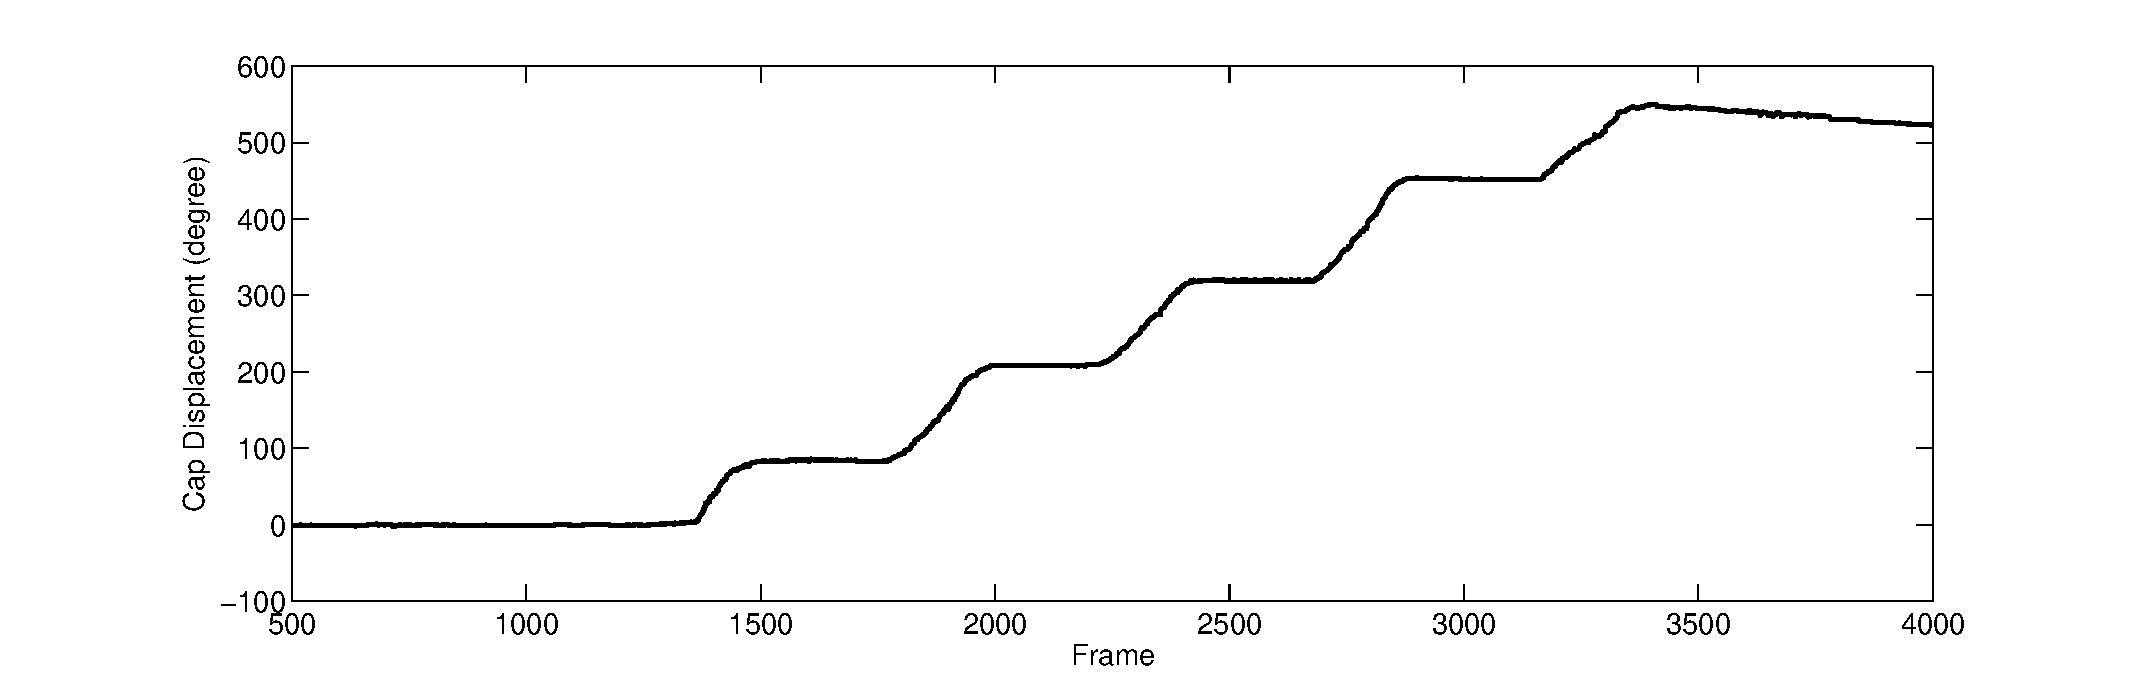
\includegraphics[width=13cm]{./fig/b3c2_5_s.eps}}
%  %\caption{ \scriptsize{Tracking cap displacement. (a) OptiTrack markers. (b) }}
%  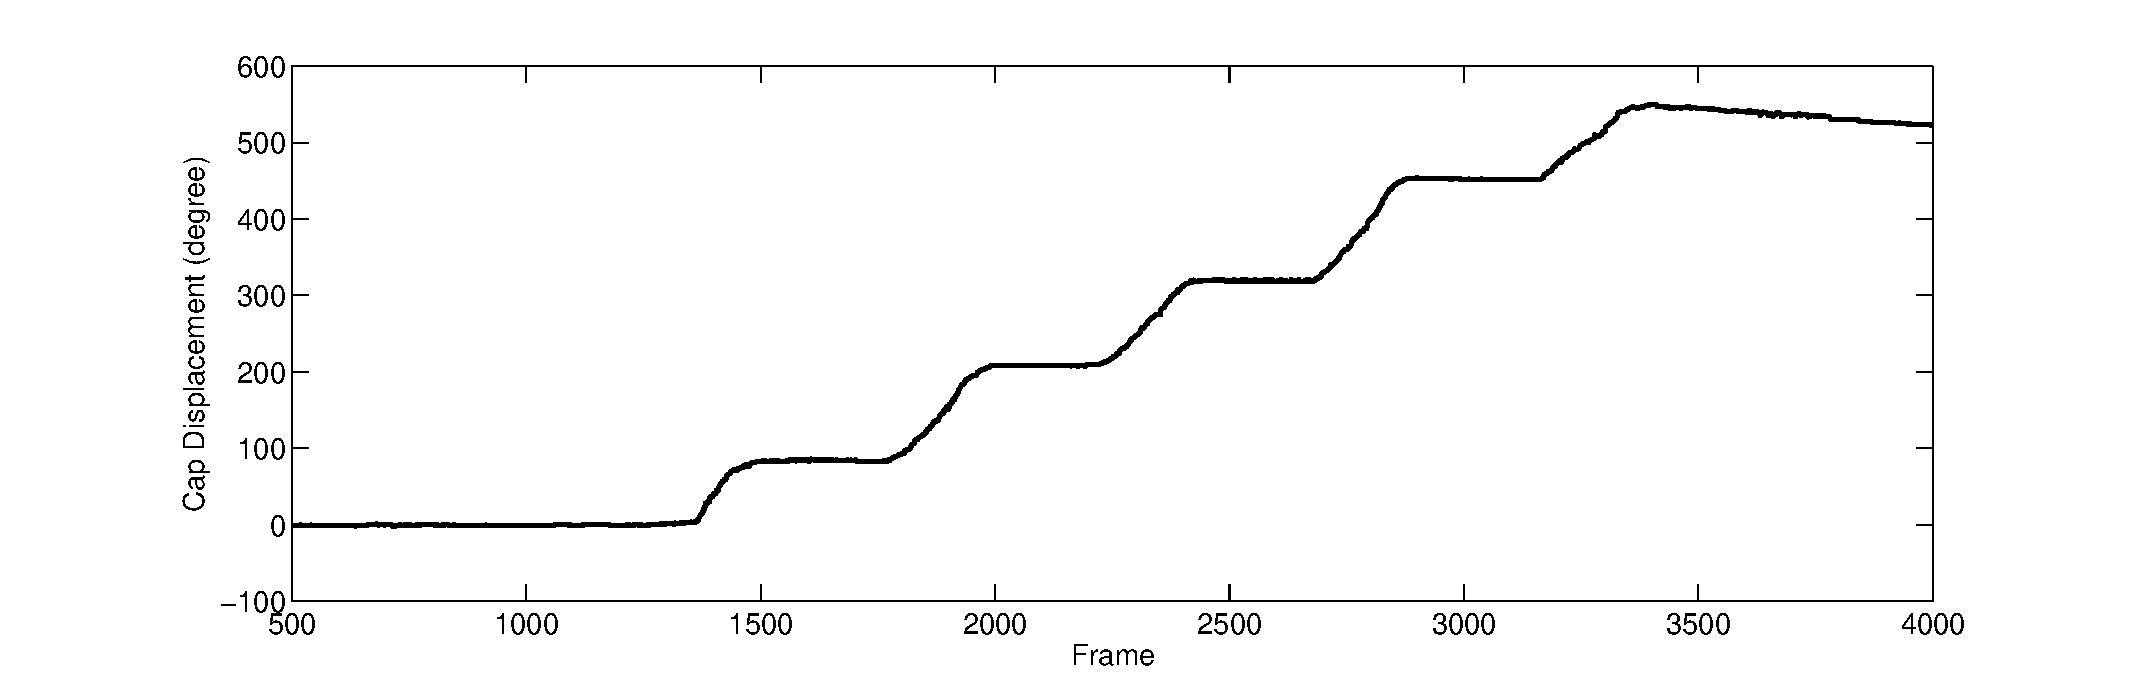
\includegraphics[width=8cm]{./fig/b3c2_5_s.eps}
%  \caption{\scriptsize{Cap angular displacement during one demonstration (of b3c2). }}
%\label{fig:optitrack}
%\end{figure}



%\begin{figure}
%  \centering
%  %\includegraphics[width=4cm]{./fig/Nano25-E.jpg}
%  %\vspace{0.2cm}
%  %\subfloat[\scriptsize{}]  {\includegraphics[width=13cm]{./fig/b3c2_5_T.eps}}
%  \includegraphics[width=8cm]{./fig/b3c2_5_T.eps}
%  %\caption{ \scriptsize{Force torque sensor. (a) Nano25-E force torque sensor. (b) Exerted torque during one demonstration (of b3c2). }}
%  \caption{ \scriptsize{Exerted torque during one demonstration (of b3c2). }}
%\label{fig:ftsensor}
%\end{figure}

\paragraph{\textbf{Grip Force}}
\label{tekscan}
As mentioned in previous section, we used two sets of Tekscan to cover
the front and the side of the human hand. This enables the
demonstrator to use any grasp they like for the task --- the human was
not restricted to using just two or three fingers as is the case in
most other grasping experiments. For each type of grasp, the reading
from the patches contacting with the cap are summed and multiplied by
their surface area to compute the total grip force. % (Figure~\ref{fig:ftsensor}).

%\begin{figure}
%  \centering
%  %\includegraphics[width=5cm]{./fig/texscan2.jpg}
%  %\hspace{0.2cm}
%  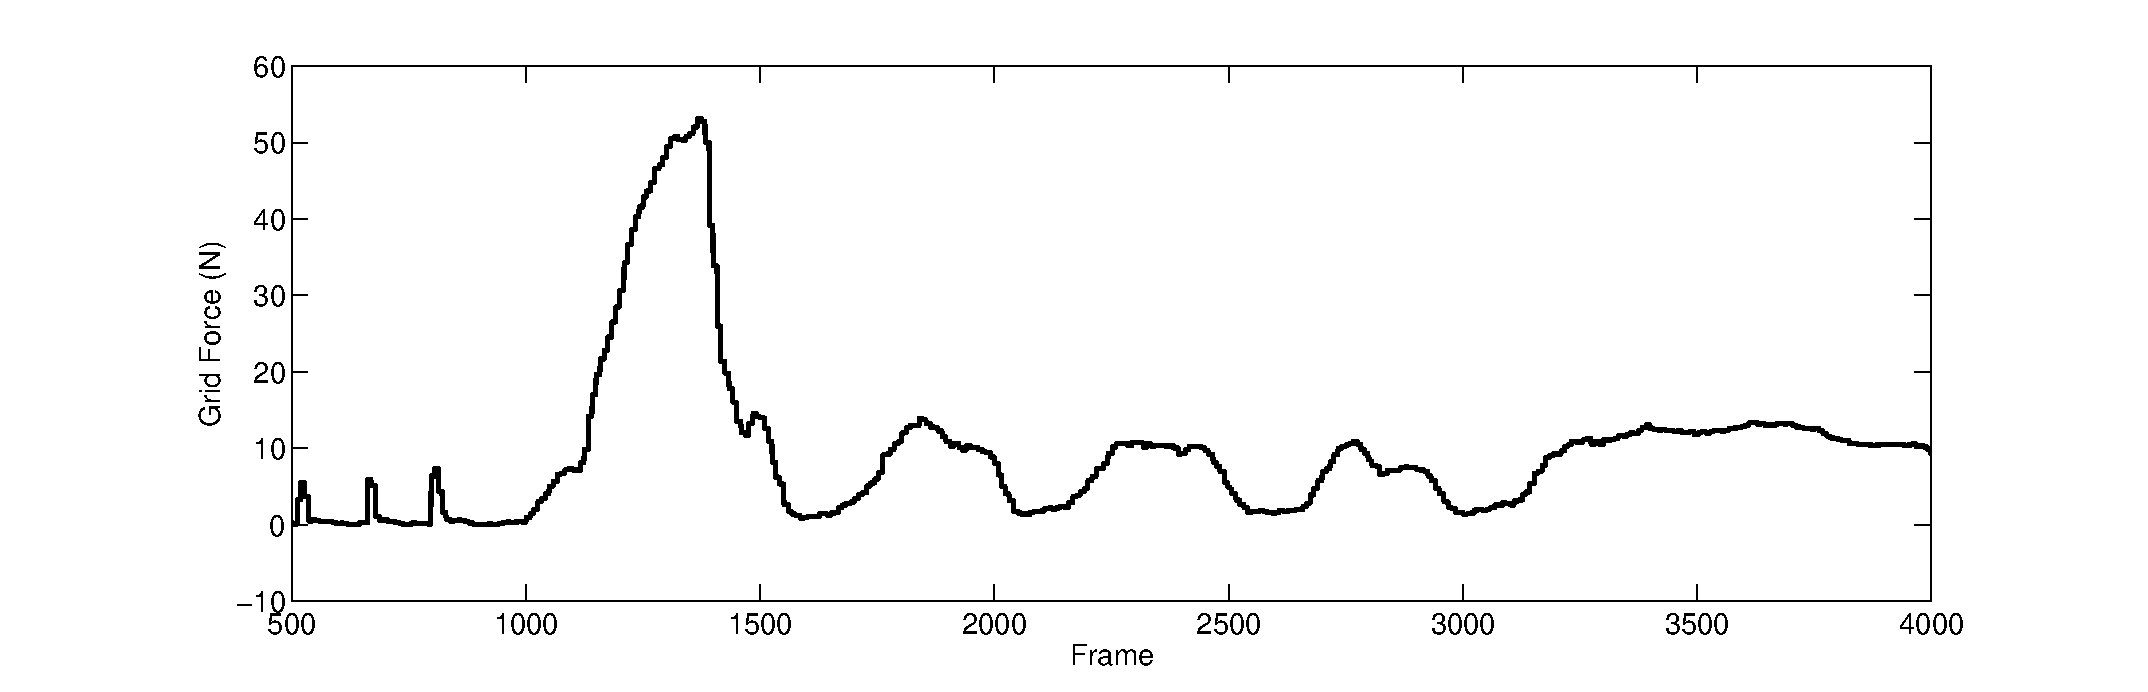
\includegraphics[width=8cm]{./fig/b3c2_5_F.eps}
%  %\caption{ \scriptsize{Tracking cap displacement. (a) Tekscan mounted on a glove. (b) Total grib force applied by different parts of the fingers in on demonstration. }}
%  \caption{ \scriptsize{Total grib force applied by different parts of the fingers in one demonstration  (of b3c2). }}
%\label{fig:ftsensor}
%\end{figure}

Data from these three channels is synchronized by aligning the
synchronization pulses. The time of the last detected pulse is set as
the zero-reference point. \textcolor{red}{After synchronization we re-sample all the
temporal sequences to 1000Hz. Thus each single data point is
synchronized. Finally, we filter the noise by a low pass
filter (200Hz).} Figure~\ref{fig:3channels} shows an example of the data from
three different channels.



\begin{figure}
  \centering
  \hspace{-0.5cm}
  \includegraphics[width=9cm]{./fig/b3c2_1_sTF.pdf}
  \vspace{-0.5cm}
  \caption{ \scriptsize{Aligned data of all three
      channels. Highlighted parts mark the turning process: blue
      blocks denote the first cycle (phase I), and green
      blocks denote the later cycles, (phase II). Phase I is
      significantly different from phase II}
}
\label{fig:3channels}
\end{figure}

% Only turning cycle
In this task we focus on the turning stage of each cycle. More
specifically, we focus on the data starting from the moment that the
fingers contact the cap and ending at the moment that the turning is
finished and the cap is released. The reaching and releasing cycles do
not involve contact with the environment and hence are not addressed
here.
% segmentation is not our job
% JJB "signal" is very different from "single"
In order to collect data from only the turning cycles, we trim the
data by the contact signal: only parts of the sequence with non-zero
contact force will be kept.\footnote{In this task the segmentation is
  done manually. The data can also be segmented by other algorithms
  but here we do not focus on task segmentation.} The trimmed
sequences are labeled by their associated equipment setup and the
order in which they occur, e.g. the first cycle of the bottle~1 with
cap~3 is labeled by $b1c3\_1$.

As can be seem from Figure~\ref{fig:3channels}, there are dramatic
difference between cycle one (the first cycle) and the rest of the
cycles: the exerted force and torque are much higher in the first
cycle. This is caused by the difference between the static friction
and the kinetic friction of the bottles. At the beginning of the task
we have to first break the contact between the bottle and the cap. The
friction we need to break at this stage is determined by the
static~FCO. Once the cap starts to move, the FCO between bottle and
cap transitions to kinetic~FCO, which is usually smaller than the
static~FCO for the same surface conditions. As a result, the torque and
hence the grip force required to turn the cap decreases in the later
cycles. This phenomenon implies that at lease two modules are needed
for this task. In the later section we will discuss these two phases
separately and referring the cycle one as ``phase I'' and the later cycles
as ``phase II''.
%JJB you need to mention this in the methods
%section under ``modular decomposition'', and then give a reference to
%this fuller description.  It is {\em not} OK to say you are telling
%the full story of the decomposition and then launch another level in
%another section. %JJB

In different demonstrations, the number of cycles used to open the cap is different, varying from four to six. The pattern of the later
cycles are similar as the demonstrator just repeats the same strategy for rotating the cap. For training, we take the first four cycles from each of the demonstrations. As mentioned above, human demonstrate the task in seven different setups, each for three times. This results in 84~time series in total for the learning.

%% what was recorded
%In each demonstration, data from first time the hand grab the cap to the cap is finally open and lifted, was record. Opening bottle cap is a cyclic task, each cycle of which includes reaching, turning and releasing stages. Depending on the tightness of the cap, a few cycles need to be done before the bottle is open. In this task we focus on the turning stage of each cycle, which start from the time that the fingers contact the cap and end at the moment that the turning is finished and the cap is released. During the turning cycles, force and torque are applied to the cap in order to break it's contact with the the bottle and the dynamics of the system changes diametrically. Our goal is to learn a model to encode human's strategy to cope with the abruptly changing environment during the turning cycle. The reaching and releasing cycles do not involve contact with the environment and hence we omit them.







\subsection{Learning Modules}
\label{learning}
%\begin{itemize}
%  \item First hierarchical clustering \ldots
%  \item Find out number of models \ldots
%  \item Second build GMM for each of the model \ldots
%\end{itemize}

In this section, we explain how we encoded the training data into just
a few different modules. As explained in Section~\ref{sec:learn}, the
first step is to cluster the data and find out the number of modules
required in this task.

\subsubsection{Data clustering}
To cluster the 84 time series $Q\{s,\tau,F\}$ obtained from human
demonstration, we first compute the distance between each pair of
series by the DTW technique. As this task is time independent,
``warping'' of the data in the dimension of time does not affect the
control policy encoded in the time series. The distances between each
pair of the time series is shown in the heatmap
(Figure~\ref{fig:heatmap}). As can be observed from the heatmap, the
trials with the same setup and in the same cycle are very similar to
each other. Hence we regard these trials representing the same control
strategy and use their variance as the threshold of the
clustering. \textcolor{red}{Trails with distance less than this threshold are considered to be in the same cluster. This is to say, our clustering is based on the assumption that trials with the same setup and in the same cycle are governed by the same control strategy. This assumption help us further cluster the large amount of data to a small number of groups.} From this heatmap we can also see that within the same
cycle, the trials with the same bottle but with different caps,
e.g. $b3c1, b3c3$ and $b3c4$, are similar to each other. In the first
cycle, the trials with the same cap but with different bottles,
e.g. $b1c3, b2c3, b3c3$ and $b4c3$, are significantly different from
each other. In the later cycles, this difference decreases
gradually. This result shows that in the opening-bottle-cap task, the
surface condition between the bottle and the cap plays an important
role in the control strategy, while the role of cap size is relatively
minor. Figure~\ref{fig:cappatterns} shows three trials of opening
bottle $b2$ with different sizes of caps. It can be seen that their
patterns are similar.

\begin{figure*}
\label{heatmap}
  \centering
  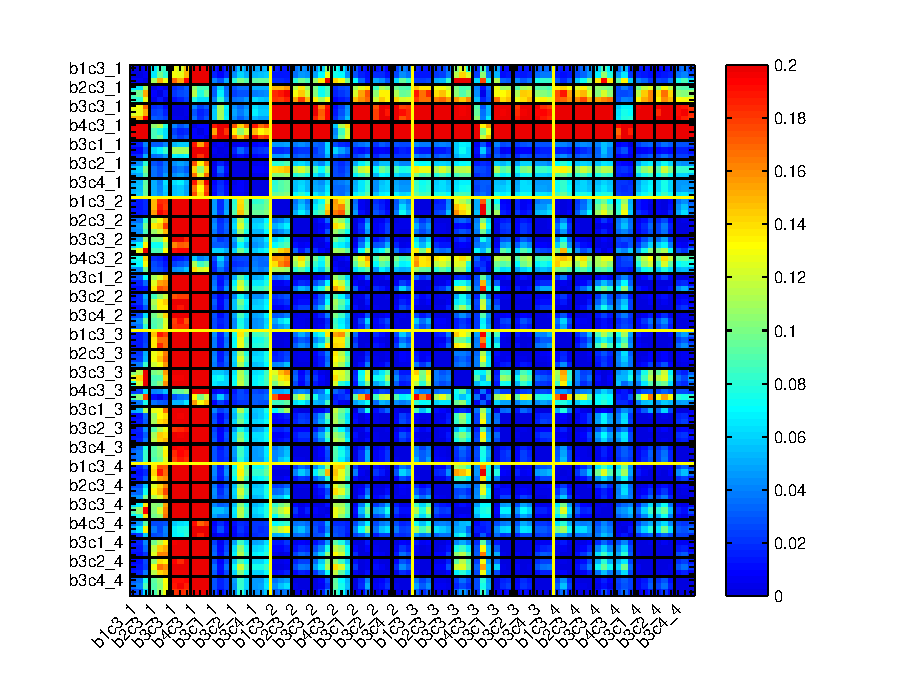
\includegraphics[width=18cm,height=18cm]{./fig/heatmap_all6_3.eps}
  \caption{ \scriptsize{A heatmap representation of the distance
      matrix of 84~time series (7~setups $\times$ 4 ~ycles $\times$
      3~trials). The labels are in the format of
      ``setup$\_$cycle''. For example, ``b1c3$\_$1'' represents the
      first cycle of the $b1c3$ setup. The yellow lines divide the x
      and y axis by the 4~cycles and hence form 16~large blocks. In
      each block, the black lines divide the x~and y~axis by the
      7~experimental setups and hence form 49~smaller blocks }  }
\label{fig:heatmap}
\end{figure*}

\begin{figure}
    \centering
    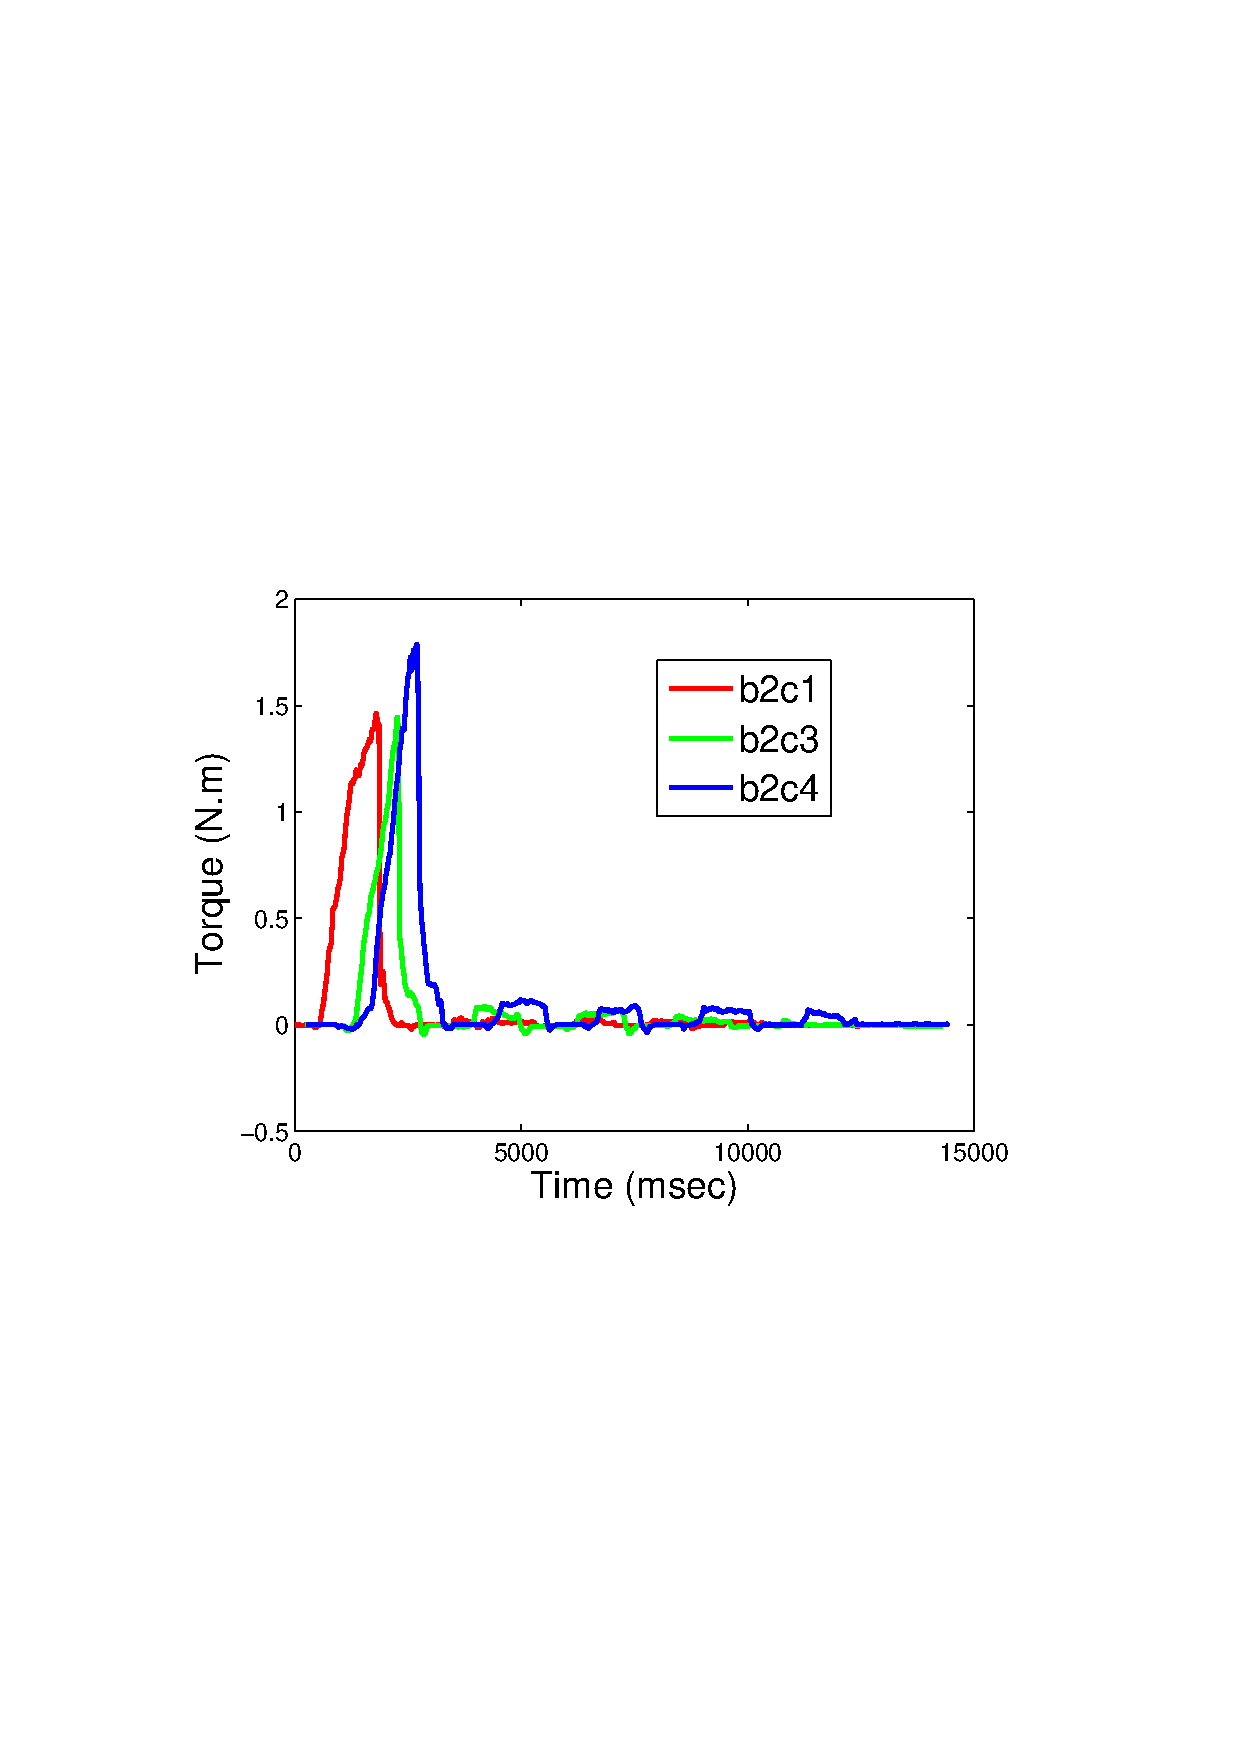
\includegraphics[width=8cm]{./fig/c1c3c4_time_T.pdf}
    \caption{ \scriptsize{Exerted torque for opening bottle $b3$ with three different cap sizes}
}
\label{fig:cappatterns}
\end{figure}


As mentioned before, the demonstration of each setup is repeated three
times. Those three time series from the same setup and same cycle are presumed to
belong to the same group. To set a threshold for clustering, we
check the distances between the three time series in the same group. The largest distance we found is 0.04
(normalized) from the $b3c2$ phase~4. We add a $10\%$ margin on this
(resulting to 0.044) and use it as the threshold of
clustering. Time-series distances less than the threshold are grouped
into the same cluster. We use hierarchical agglomerative
clustering (Section~\ref{sec:cluster}) to merge the data into
fewer clusters. After five mergings, the clusters are no longer
mergeable and three clusters remains.

These three clusters contain the data from:

\begin{enumerate}
\item phase I of $b4c3$ (most difficult bottle), 3 time series;
\item phase I of $b3c1, b3c2, b3c3, b3c4, b2c3$ and phase II of $b4c3$, 24 time series;
\item phase I of $b1c3$ (easiest bottle) and phase II of the other setups, 57 time series.
\end{enumerate}

The result of clustering is shown in Table~\ref{tab:cluster}. This
result suggests that humans use three different strategies for opening
bottles: one for handling phase~I of the most difficult bottle with
adhesive materials on the bottle and cap surfaces; one for handling
phase~I of most bottles and phase~II of the most difficult bottle; and
one for handling phase~I of the lubricated bottle and phase~II of the
other bottles. The size of the cap turns out to be play a less
important role in the control strategies. According to these results, we
encode these three clusters separately.


%\begin{table}
%\centering
%\renewcommand{\arraystretch}{1.5}
%    \begin{tabular}
%    %{|>{\centering\arraybackslash}p{2cm}|>{\centering\arraybackslash}p{1.2cm}|>{\centering\arraybackslash}p{1.7cm}|>{\centering\arraybackslash}p{1.2cm}|>{\centering\arraybackslash}p{1.5cm}|>{\centering\arraybackslash}p{1.5cm}|>{\centering\arraybackslash}p{1.7cm}|>{\centering\arraybackslash}p{1.7cm}|>{\centering\arraybackslash}p{0.9cm}|}
%    { | c |>{\centering\arraybackslash}p{10cm}|}
%    \hline
%    Cluster & Member time series \\ \hline
%    1       & $b4c2_1$  \\ \hline
%    2       & $b2c2_1,b3c2_1,b4c2_2,b4c2_3,b4c2_4,b2c3_1,b2c4_1$  \\ \hline
%    3       & $b1c2_1,b1c2_2,b1c2_3,b1c2_4,$
%             $  b2c2_2,b2c2_3,b2c2_4, $ \\
%    &         $  b3c2_2,b3c2_3,b3c2_4, $
%            $  b2c1_2,b2c1_3,b2c1_4, $ \\
%    &         $  b2c3_2,b2c3_3,b2c3_4, $
%             $  b2c4_2,b2c4_3,b2c4_4$  \\ \hline
%    \end{tabular}
%\caption{Clustering result}
%\label{tab:cluster}
%\end{table}


\begin{table*}
\centering
\caption{Clustering results}
\begin{tabular}{p{1.4cm} p{1.4cm}|p{1.6cm} p{1.6cm} p{1.6cm}  p{1.6cm} }
& & \parbox[c]{1em}{\includegraphics[width=1.5cm]{./fig/c1.jpg}}\newline Cap 1
& \parbox[c]{1em}{\includegraphics[width=1.5cm]{./fig/c2.jpg}}\newline Cap 2
& \parbox[c]{1em}{\includegraphics[width=1.5cm]{./fig/c3.jpg}}\newline Cap 3
& \parbox[c]{1em}{\includegraphics[width=1.5cm]{./fig/c4.jpg}}\newline Cap 4      \\ \hline
{\parbox[c]{1em}{\includegraphics[width=1.5cm]{./fig/b1.jpg}}}
         & Phase I  &           &           & {\vspace{-0.7cm}}\pbox{2cm}{(b1c3) \\ Cluster 3} &           \\
Bottle 1 & Phase II &           &           &        Cluster 3 &           \\ \hline
{\parbox[c]{1em}{\includegraphics[width=1.5cm]{./fig/b2.jpg}}}
%         & Phase I  &{\vspace{-0.7cm}}\pbox{2cm}{(b2c1) \\Cluster 2} &{\vspace{-0.7cm}}\pbox{2cm}{(b2c2) \\Cluster 2} &{\vspace{-0.7cm}}\pbox{2cm}{(b2c3) \\Cluster 2} &{\vspace{-0.7cm}}\pbox{2cm}{(b2c4) \\Cluster 2} \\
%Bottle 2 & Phase II &       Cluster 3 &       Cluster 3 &       Cluster 3 &       Cluster 3 \\ \hline
         & Phase I  &           &           &{\vspace{-0.7cm}}\pbox{2cm}{(b2c3) \\Cluster 2} &           \\
Bottle 2 & Phase II &           &           &       Cluster 3 &           \\ \hline
{\parbox[c]{1em}{\includegraphics[width=1.5cm]{./fig/b3.jpg}} }
%         & Phase I  &           &           &{\vspace{-0.7cm}}\pbox{2cm}{(b3c3) \\Cluster 2} &           \\
%Bottle 3 & Phase II &           &           &       Cluster 3 &           \\ \hline
         & Phase I  &{\vspace{-0.7cm}}\pbox{2cm}{(b3c1) \\Cluster 2} &{\vspace{-0.7cm}}\pbox{2cm}{(b3c2) \\Cluster 2} &{\vspace{-0.7cm}}\pbox{2cm}{(b3c3) \\Cluster 2} &{\vspace{-0.7cm}}\pbox{2cm}{(b3c4) \\Cluster 2} \\
Bottle 3 & Phase II &       Cluster 3 &       Cluster 3 &       Cluster 3 &       Cluster 3 \\ \hline
{\parbox[c]{1em}{\includegraphics[width=1.5cm]{./fig/b4.jpg}}\newline }
         & Phase I  &           &           &{\vspace{-0.7cm}}\pbox{2cm}{(b4c3) \\Cluster 1} &           \\
Bootle 4 & Phase II &           &           &       Cluster 2 &           \\ \hline
\end{tabular}
\label{tab:cluster}
\end{table*}

%\begin{figure}
%\label{forcecluster}
%  \centering
%  \includegraphics[width=11cm]{./fig/forcecluster.jpg}
%  \caption{ \scriptsize{Hierarchal clustering result.}
%}
%\end{figure}

\subsubsection{Learning Modules}
\label{sec:module}
We encode the data in each of the modules by means of GMM. As
explained in Section~\ref{sec:model}, a forward model and an inverse
model are built for each module. The forward model is encoded by the
joint distribution $p\{s_t,s_{t-1},a_{t-1}\mid\Omega_F\}$, while the
inverse model is encoded by
$p\{s_t,s{t+1},a_t,a_{t-1}\mid\Omega_I\}$. For each model, the number
of Gaussians is determined by the Bayesian information criterion
(BIC). We use 25 Gaussian for cluster 1, 40 for cluster 2 and 15 for
cluster 3. The BIC tests for each module / cluster are shown in
Figure~\ref{fig:bic}.

\begin{figure}
  \centering
  \subfloat[\scriptsize{Cluster 1. Optimal number of Gaussians is 25.}]{\includegraphics[width=6cm]{./fig/bic_cluster1_2.eps}}

  \subfloat[\scriptsize{Cluster 2. Optimal number of Gaussians is 40.}]{\includegraphics[width=6cm]{./fig/bic_cluster2_2.eps}}

  \subfloat[\scriptsize{Cluster 3. Optimal number of Gaussians is 15.}]{\includegraphics[width=6cm]{./fig/bic_cluster3_2.eps}}

  \caption{ \scriptsize{BIC test results for clusters, determining the
      number of gaussians used in each module }
}

\label{fig:bic}
\end{figure}

%\begin{table}
%\centering
%\renewcommand{\arraystretch}{1.5}
%    \begin{tabular}
%    %{|>{\centering\arraybackslash}p{2cm}|>{\centering\arraybackslash}p{1.2cm}|>{\centering\arraybackslash}p{1.7cm}|>{\centering\arraybackslash}p{1.2cm}|>{\centering\arraybackslash}p{1.5cm}|>{\centering\arraybackslash}p{1.5cm}|>{\centering\arraybackslash}p{1.7cm}|>{\centering\arraybackslash}p{1.7cm}|>{\centering\arraybackslash}p{0.9cm}|}
%    { | c | c | c | c | c |}
%    \hline
%    Cluster & Forward Model &  Inverse Model \\ \hline
%    1       & 98.1\%  & 13.8     \\ \hline
%    2             & 92.1\%  & 21.9    \\ \hline
%    3              & 91.0\%  & 16.0    \\ \hline
%    \end{tabular}
%\caption{Number of Gaussians in each GMM}
%\label{tab:GMM}
%\end{table}


\subsection{Generating robot motor commands for manipulation}
\label{sec:command}
Our approach is independent of robot system and can potentially be
applied to any robot. We chose to implement this work with a Barrett
hand mounted on a KUKA lightweight robot as these were available in
our lab. We implemented the multiple module system on this platform to
enable the robot to open bottle caps.

\begin{algorithm}
  \caption{Control Algorithm}
  \begin{algorithmic}[1]
    \For{r = 1:4}
    \State REACHING(): Robot moves to the initial position\;
        \Function{TURNING()}{} %      \Comment{$\oplus$: bit}
          \State Read previous sensor information $\{s_{t-1},\tau_{t-1},F_{t-1}\}$\;
          \For{k=1:3}
            \State $\hat{s}^{k}$ = FORWARD($s_{t-1},T_{t-1},\Omega_I^k$) \;
          \EndFor
          \For{k=1:3}
            \State $\lambda{k}$ = ResponsibilityFactor($\hat{s}^{k},s_t$) \;
          \EndFor
          \State Read current sensor information $\{s_{t}\}$\;
          \For{k=1:3}
            \State $\{a^k\}$ = INVERSE($s*_{t+1},s_t,a_{t-1}$) \;
          \EndFor
          \State $\{a_t\} = \sum_{k=1,2,3}\lambda{k}\{a^k\}$\;\;
          \State Add compensating torque to $\tau_t$\;
          \State Execute motor command $\{a_t\}$ \;
          \State RELEASING(): Release the cap;
        \EndFunction
    \EndFor

    \While{LIFTCAP() is false}
        \State REACHING();
        \State TURNING();
        \State RELEASING();
    \EndWhile

  \end{algorithmic}
  \label{code:control}
\end{algorithm}


In this experiment, we control the wrist joint (last joint of the KUKA)
for producing torque to turn the bottle cap. A force torque sensor is
fixed under the bottle to provide torque feedback. Each finger of the
Barrett hand is mounted with a
$Syntouch$\footnote{http://www.syntouchllc.com/} tactile sensor, which
is calibrated to provide contact force information, for the grip force
feedback. The cap displacement is measured by the wrist joint
displacement, assuming that there is no slippage between the fingers and
the cap.

The target bottle is fixed on the top of a table with its cap
tighten. The robot is placed above it at a distance that allows a
proper grasp on the cap. The Barrett hand then closes the fingers until
the bottle cap is touched. This position is recorded as the initial
position, where the cap displacement is marked as zero. In the
experiment we focus on the turning cycle. The releasing and reaching
cycles are programmed by opening the fingers and restoring to the
initial position. \textcolor{red}{ The information gathered from the Tekscan during the demonstrations is transferred to the Syntouch and used to guide the grip force. During the process, the tactile sensors are used to ensure the fingers are touching the cap and providing enough grip force to avoid slide between the hand and the cap.}

% JJB check:  I added the lambdas in here to reference back to
% equation 10.   Check that this makes sense?
We first tested the model with the trained bottles and then with two
new bottles. With each bottle, the turning-releasing-restoring cycles
are repeated four times. Data streams from the sensors are filtered to
$100Hz$. Once the turning cycle starts, the forward models take the
torque and displacement at the last time step as input, compute the
expected displacement of the current time step. These expected
displacements are compared with the actual displacement measured at
the sensor to evaluate the reliability, expressed as a normalized
responsibility factor ($\lambda_t^k$), of each module ($k$). The inverse models
take the current displacement, desired next displacement, and the
previous torque as input to compute the a proper action
(torque) to take on the cap. Each of the three outputs is weighted by
multiplied with its responsibility factor, and the final output is the sum of the three weighted outputs (Algorithm~\ref{code:control}).

In the process of implementation on a real robot, we found that
without putting any restriction of the responsibility factor, it can
change very rapidly. This is caused by the environmental noise in the
sensory input and results in instability of the control system. We
therefore apply a low-pass filter \textcolor{red}{(100 Hz)} on the responsibility factor
$\lambda_t^k$ to reduce the fluctuation. \textcolor{red}{This filtering implies that
the real dynamics do not switch back and forth with high frequency, which is consistent
with the character of our task.} %(Figure~\ref{fig:rf}).

%\begin{figure}
%  \centering
%  \includegraphics[width=2cm]{./fig/void.jpg}
%  \caption{ \scriptsize{Filtered responsibility factor. (TODO)}
%}
%\label{fig:rf}
%\end{figure}

% "lag" is not "slag"
Before applying the final output on the robot, a compensational torque is added to it in order to compensate the lag causing by the distortion of the robot hand during turning. The control algorithm described above is shown in algorithm~\ref{code:control}.


\subsection{Experiment results}


% TODO:
% 1) explain whether the use of the clusters correspond to your expectations and really relate to an identification of different phases
% 2) what the novel object consist of, in what do they differ from the other objects
% 3) what were your expectations in terms of cluster use for these new objects
% 4) Do the results match your expectations

%We implement this algorithm with two bottles (b1 and b4) in the training set and then two bottles (b5 and b6) had not been used for training.
We validated the algorithm to control cap opening in our robot. We
first tested the ability of the system to open 2 of the bottles seen
during training ($b1$ and $b4$). We then tested the generalization
capacity of the system by opening two bottles ($b5$ and $b6$) not seen
during training.  Bottle $b1$ and $b4$ are the easiest and most difficult
bottle to open in the training set.  Bottle $b5$ is a large bottle,
which is hard for human to grasp and open. Bottle $b6$ is a glass bottle
with a plastic cap. The surface interaction between these two
materials had not been demonstrated. As the Barrett hand is
significantly larger than a human hand, $b1, b4, b6$ are mounted with
$c5$ (the cap of $b5$ with diameter $110 mm$) on the top to ensure a
firm grasp. In total, four different setups were used in the
experiment: $b1c5, b4c5, b5c5$ and $b6c5$. As discuss above, the size
of the cap has minor effect on the control strategy. Therefore we
expected the setups $b1c5$ and $b4c5$ to result in similar behavior as
those of $b1c3$ and $b4c3$ in the training. The experimental results
and demonstration snapshots are shown in
figures~\ref{fig:demo_b1}-~\ref{fig:demo_b6}~\footnote{Demonstration
  videos are available at http://www.cs.bath.ac.uk/~bh325/opencap.rar
  and will be provided as an electronic supplement to the
  article.}. Figure~\ref{fig:demo_b1b4b5b6} is a similar plot to the
figure from the demonstration, figure~\ref{fig:bottlepatterns}, which
aligns the exerted torque of the four experiments. %JJB check all the
                                %above is OK. JJB

In each experiment we record the cap displacement, exerted torque, and
the responsibility factors of all three modules. Bottle $b1$ is the
easiest bottle to open in the training set, the control policies of
both phase~I and phase~II are grouped into cluster~3. As a result,
in the $b1$ experiment, module~3 takes most of the responsibility
(Figure~\ref{fig:demo_b1}).

%its != it's.  It's is also informal and never occurs in academic papers.
Bottle $b4$ is the most difficult bottle to open in the training set
and its phase~I requires more than $3Nm$
(Figure~\ref{fig:bottlepatterns}). Due to the smooth contact surfaces
between the Barrett hand and the cap, it is difficult to apply $3Nm$
torque to the cap without slipping. To avoid damaging the robot, we
tested $b4$ phase~II only: the cap is loosely screwed on the
bottle. Without knowing this, in the experiment the robot is able to
properly estimate the current task context. As can be seen from the
figure~\ref{fig:demo_b4}, which is different from $b1$, the dominant
module is module~2 which corresponds to  $b4$, phase~II. This
performance would be hard to achieved with a deterministic system based
on expected values for friction coefficients.

Bottle $b5$ is a novel one but is made of a similar material (plastic) to
the training bottles. A very similar torque profile to $b2$ and $b3$ is
generated for $b5$: phase~I is sharp, while phase~II is flatter and
significantly smaller than phase~I ($b2$:
Figure~\ref{fig:bottlepatterns}, $b3$: Figure~\ref{fig:cappatterns},
$b5$: Figure~\ref{fig:demo_b5}). This is because $b5$ has a dry contact
surface as $b2$ and $b3$, and $b1$ is lubricated and $b4$ is attached with
a sticky material, honey.

Bottle $b6$ is also a novel one but with novel surface materials
(plastic and glass)\footnote{A common way of measuring the FCO of a
  material is measuring it against metal: the static FCO between glass
  and metal is 0.5--0.7, while between two polythene and steel is
  around 0.2. This implies that the plastic and glass are indeed very
  different in FCO. There is not a universal measurement of the FOC
  between plastic and glass.}. Its torque profile is different from
what we observed in training set. Despite this, $b6$ is opened with this
torque profile generated by the three learnt modules.

\textcolor{red}{In these experiments, the robot always choose to use the combination of modules. At one hand, this is because of the variance of the forward models. The variance of a GMM represents the variance of the training data, i.e. human demonstrations, and a GMM can have locally large variance.
In our approach, each GMM is learned independently, without knowing the boundaries of other modules. This can result in a GMM having non-zero probability at the borders of other modules. At the other hand, more importantly, the way we compute the responsibility factor is one that encourages more cooperation between modules. In this way, we can generalise better to novel task contexts, as more modules will contribute to generate new motor commands. As can be seen from the results, our method can generate commands properly to accomplish the task in both trained and novel task contexts. Other ways of computing the responsibility factor that bring less cooperation may cause instability when generalise to new task contexts. }


With the above four different setups, the modular model adapts
accordingly and successfully generates torque commands to open the
bottles. Successful cap opening is achieve when the cap is unscrewed
far enough that it can be lifted up. Though no prior information is
provided about the bottles, the task contexts are properly estimated
and ``contextualized'' motor commands are generated to unscrew the
caps. These experiments show that our multiple modular approach is
indeed effective in manipulation tasks.
%JJB: "contextualized" is
                                %spelled right (US spelling as you've
                                %been using that.)  Emacs / ispell
                                %doesn't recognise it though.



% JJB: don't call the experiments with the robot "demonstrations", that
% will confuse people. Only the humans are doing demonstrations in
% this context.  The robots are performing.  Of course it could also
% be seen as a demonstratoin of our technique, but you need to
% restrict how you use the word so that people don't get confused.
% This is common in technical writing.
\begin{figure*}
  \centering
  \vspace{0.8cm}
  \subfloat[\scriptsize{Snapshots from the robot opening bottle~ $b1$}]
  {\includegraphics[width=13cm]{./fig/demo_b1.jpg}}

  \vspace{0.3cm}
  %\hspace{0.2cm}
  \subfloat[\scriptsize{Cap displacement during the robot's opening}]
  {\includegraphics[width=13cm]{./fig/demo_b1_s.eps}}

  \vspace{0.3cm}
  \hspace{-0.3cm}
  \subfloat[\scriptsize{Torque exerted by the robot against cap displacement}]
  {\includegraphics[width=13cm]{./fig/demo_b1_T.eps}}

  \vspace{0.3cm}
  %\vspace{0.5cm}
  \subfloat[\scriptsize{Responsibility factor against cap
    displacement, for each module}]
  {\includegraphics[width=13cm]{./fig/demo_b1_rf.eps}}
  \caption{ \scriptsize{The robot opens bottle~$b1$.}
}

\label{fig:demo_b1}
\end{figure*}

\begin{figure*}
  \centering
  \vspace{0.8cm}
  \subfloat[\scriptsize{Snapshots from the robot opening bottle~$b4$}]
  {\includegraphics[width=13cm]{./fig/demo_b4.jpg}}

  \vspace{0.3cm}
  %\vspace{0.5cm}
  \subfloat[\scriptsize{Cap displacement during the robot's opening}]
  {\includegraphics[width=13cm]{./fig/demo_b4_s.eps}}

  \vspace{0.3cm}
  \hspace{-0.2cm}
  \subfloat[\scriptsize{Torque exerted by the robot against cap displacement}]
  {\includegraphics[width=13cm]{./fig/demo_b4_T.eps}}

  \vspace{0.3cm}
  %\vspace{0.5cm}
  \subfloat[\scriptsize{Responsibility factor against cap displacement, for each module}]
  {\includegraphics[width=13cm]{./fig/demo_b4_rf.eps}}

  \caption{ \scriptsize{The robot opens bottle~$b4$}
}
\label{fig:demo_b4}
\end{figure*}

%JJB --- fix the captions for the below as I already did for the
%above. %JJB
\begin{figure*}
  \centering
  \vspace{0.8cm}
  \subfloat[\scriptsize{Snapshots for robot opening bottle~b5 demonstration}]
  {\includegraphics[width=13cm]{./fig/demo_b5.jpg}}

  \vspace{0.3cm}
  %\vspace{0.5cm}
  \subfloat[\scriptsize{Cap displacement during the robot's opening}]
  {\includegraphics[width=13cm]{./fig/demo_b5_s.eps}}

  \vspace{0.3cm}
  %\vspace{0.5cm}
  \subfloat[\scriptsize{Torque exerted by the robot against cap displacement}]
  {\includegraphics[width=13cm]{./fig/demo_b5_T.eps}}

  \vspace{0.3cm}
  %\vspace{0.5cm}
  \subfloat[\scriptsize{Responsibility factor against cap     displacement, for each module}]
  {\includegraphics[width=13cm]{./fig/demo_b5_rf.eps}}

  \caption{ \scriptsize{The robot opens bottle~$b5$}
}
\vspace{5cm}
\label{fig:demo_b5}
\end{figure*}

\begin{figure*}
  \centering
  \vspace{0.8cm}
  \subfloat[\scriptsize{Snapshots for robot opening bottle~b6 demonstration}]
  {\includegraphics[width=13cm]{./fig/demo_b6.jpg}}

  \vspace{0.3cm}
  %\vspace{0.5cm}
  \subfloat[\scriptsize{Cap displacement during the robot's opening}]
  {\includegraphics[width=13cm]{./fig/demo_b6_s.eps}}

  \vspace{0.3cm}
  \hspace{-0.5cm}
  \subfloat[\scriptsize{Torque exerted by the robot against cap displacement}]
  {\includegraphics[width=13cm]{./fig/demo_b6_T.eps}}

  \vspace{0.3cm}
  %\vspace{0.5cm}
  \subfloat[\scriptsize{Responsibility factor against cap     displacement, for each module}]
  {\includegraphics[width=13cm]{./fig/demo_b6_rf.eps}}

  \caption{ \scriptsize{The robot opens bottle~$b6$}
}
\label{fig:demo_b6}
\end{figure*}


\begin{figure}
  \centering
  \includegraphics[width=8cm]{./fig/rb1b4b5b6_time_T.eps}
  \caption{ \scriptsize{Robot exerted torque for opening four bottles: b1 b4 b5 b6. Time is warped and shifted for displace purpose}
}
\label{fig:demo_b1b4b5b6}
\end{figure}


%A set of snapshots of the implementations are shown in Figure~\ref{fig:demo_train} and~\ref{fig:demo_new}. Figure~\ref{fig:demo_result} shows the sensory data from these demonstrations.

%\begin{itemize}
%  \item Demonstration on the learnt bottles \ldots
%  \item Demonstration on a new bottle \ldots
%  \item Filtering noise  \ldots
%  \item different module's rf
%\end{itemize}

%\begin{figure}
%  \centering
%  \includegraphics[width=13cm]{./fig/demo_train.jpg}
%  \caption{ \scriptsize{Robot demonstration on opening a trained bottle cap. (TODO)}
%}
%\label{fig:demo_train}
%\end{figure}
%
%\begin{figure}
%  \centering
%  \includegraphics[width=13cm]{./fig/demo_new.jpg}
%  \caption{ \scriptsize{Robot demonstration on opening a new bottle cap. (TODO)}
%}
%\label{fig:demo_new}
%\end{figure}
%
%\begin{figure}
%  \centering
%  \includegraphics[width=2cm]{./fig/void.jpg}
%  \caption{ \scriptsize{Robot demonstration data. (TODO)}
%}
%\label{fig:demo_result}
%\end{figure} 
\section{Conclusion and Discussion}
\label{sec:diss}
In this paper we proposed a modular approach for learning manipulation task from human demonstration. We discover the number of modules needed in a task by hierarchical clustering. From each cluster we use forward and inverse model pairs to model the motor control mechanism. The forward models predict the effect of the previous motor command, while the inverse models compute a motor command to bring the current state to a desired state. The statistical approach enables us to estimate the reliability of the inferences of each module under the current context. The final motor command is the sum of the weighed command from each module. With an object centric viewpoint, the learnt human internal models can be easily transfer to robot. Our experiment verifies that by this modular approach, the robot can automatically recognize the current task context and compute proper motor commands to accomplish a manipulation task, i.e. opening bottle caps.

%We contribute an experimental validation of this approach by learning the human strategy of opening bottle cap. This is a complex manipulation task as the friction between the contact surfaces involve extremely complicated physics. Without detail knowledge of tribology, human success to open many different bottle caps in daily life. We aim to learn this strategy by a modular approach. The human demonstrator demonstrated the task in seven different contexts and we group these demonstrates into three groups. Forward and inverse model pairs are learnt from each group for motor control.

% TODO: where is useful, where is not useful
Our approach is applicable to manipulation tasks that require adaptive control strategy. It has a few benefits compare to the pervasive methods for adaptive control, e.g. classic model identification adaptive control and reinforcement learning. By imitating the human behaviors, we do not need to derive the system dynamics nor the cost function of the tasks, which involve deep insight of the task and can be painstaking. The difficulty of modeling an adaptive strategy is further reduced by a modular approach: dividing the large state space into several subspaces, where the local strategies can be approximated more accurately. With this approach, we divide the the complex human strategy into a few modules, and combine them to generate contextized motor commands.

Our object centric approach is a practical approach for teaching a robot manipulation tasks that require proprioception. This allows human demonstrating the task with physical contact with the object, and hence have direct feedback from their own sensory system. We bypass the problem of direct mapping human movement to robot movement by expressing the strategy from an object centric viewpoint. This can largely benefit learning manipulation tasks such as impedance control task, as measuring human muscle impedance is hard while measuring the impedance of an object is more feasible.

We compute the final motor command by summing the output of each module. This makes an assumption that the state space is continuous. For tasks with discontinuous space, constraints have to be applied and the other control methods mentioned above are more applicable.

There are many promising directions of further studies of this work. The first is to apply this approach to other contact tasks and learn a more general human control strategy in handling the instability caused by friction.
%Clarify the fact here that you hardly analyze the effect of changing the cap size and the positioning of the fingers on the cap which is revealed in the tactile signature, and that this will be future work.
In this study, we focus on the control strategy of unscrewing the cap. We hardly analyze the effect of changing the cap size and the positioning of the fingers on the cap, which is revealed in the tactile signature. This analysis will be progressed in the future work to study task specific grasping strategy~\citep{el2013generation,dang2014semantic}.

To extend our approach to learn tasks involve multiple steps, one could also integrate it with task segmentation technique, to break down the task into atomic steps and recognize the steps needs modular approach. How does the number of modules change according to the tasks is another useful information to reason about.

%So far we have implement the approach with a task controlled in three dimensions and by three modules. How does the number of modules change according to the dimension of the task is another useful information to reason about.

In summary, tasks involve multiple phases or different contexts are hard to implement by a single model. Modular architecture is a practical approach for modeling these tasks. As manipulation usually involves multi-phase friction and multi-body interaction, learning manipulation tasks with a modular approach can simplify the modeling problem in a large extend.



%\begin{itemize}
%  \item Can be used in more complex robot
%  \item if slip can be detected ...
%  \item grasp the cap, studied in another experiment
%\end{itemize}

%During the task, the dynamics of the environment changes abruptly. Figure~/ref{phase12} shows an example of the recorded time sequence of the opening bottle cap task. From the 4 turning cycles we see a dramatic difference between the first cycle and the rest of the cycles. This is not surprise as in the first turning cycle we have to apply a large torque to break the contact between the cap and the bottle, i.e. to overcome the static friction. Once the contact is broken, a much smaller torque is required to rotate the cap, i.e. to overcome the kinema.tic friction.


\bibliographystyle{spbasic}
\bibliography{multimodel,jjb}
\end{document}
% end of file template.tex

